% Questo file definisce lo stile che verrà applicato
% ad ogni pagina di contenuto
\documentclass[a4paper,11pt]{article}

\usepackage{ifthen}
\usepackage[
 a4paper,
 top=2.5cm,
 bottom=2.5cm,
 left=1.5cm,
 right=1.5cm,
 head=30pt
]{geometry}
\usepackage[italian]{babel}
\usepackage[utf8x]{inputenc}
\usepackage[T1]{fontenc}
\usepackage{fancyhdr}
\usepackage[colorlinks=true, urlcolor=black, citecolor=black, linkcolor=black]{hyperref}
\usepackage{tabularx}
\usepackage{multirow}
\usepackage{booktabs}
\usepackage{color}
\usepackage[dvipsnames]{xcolor}
\usepackage{graphicx}
\usepackage{eurosym}
\usepackage{amsmath}
\usepackage{relsize}
\usepackage{placeins}
\usepackage{ltablex}
\usepackage{float}

\usepackage[multidot]{grffile}
\usepackage{xcolor,colortbl}
\definecolor{lightblue}{HTML}{56B4E6}
\definecolor{blue}{HTML}{2953A1}
\definecolor{darkblue}{HTML}{1E396E}
\usepackage{longtable}

\usepackage[toc,page]{appendix}
\renewcommand\appendixtocname{Appendice}
\renewcommand{\appendixpagename}{Appendice}

\newcommand\pagenumberingnoreset[1]{\gdef\thepage{\csname @#1\endcsname\c@page}}

% Cambia il font 
\renewcommand*\rmdefault{qhv}

% ***STILE PAGINA***
\pagestyle{fancy}
\fancyhf{}
\setlength{\headheight}{1cm} 
% No indentazione paragrafo
\setlength{\parindent}{0pt}

% ***INTESTAZIONE***
\newcommand\textline[4][t]{%
  \noindent\parbox[#1]{.333\textwidth}{\raisebox{-0.40\height}{#2}}%
  \parbox[#1]{.333\textwidth}{\centering #3}%
  \parbox[#1]{.333\textwidth}{\raggedleft #4}%
}

\lhead{
	\textline[t]{
\includegraphics[width=1cm, keepaspectratio=true]{../../../Template/Logo/Logo.png}}{\progettoShort}{\documento}
}

\renewcommand{\headrulewidth}{0.4pt}  %Linea sotto l'intestazione

% ***PIÈ DI PAGINA***
\lfoot{\textit{\gruppoLink}\\ \footnotesize{\email}}
\rfoot{\thepage} %per le prime pagine: mostra solo il numero romano
\cfoot{}
\renewcommand{\footrulewidth}{0.4pt}   %Linea sopra il piè di pagina


% Ridefinisce command \paragraph{} andando a capo ogni dopo la parola dentro le parentesi ed ha la possibiltà di enumerazione fino a n cifre modificando il numero dentro "secnumdepth"
\usepackage{titlesec}

\setcounter{secnumdepth}{7}
\setcounter{tocdepth}{7}


% Visualizza paragraph come una section
\titleformat{\paragraph}{\normalfont\normalsize\bfseries}{\theparagraph}{1em}{}
\titlespacing*{\paragraph}{0pt}{3.25ex plus 1ex minus .2ex}{1.5ex plus .2ex}

\titleformat{\subparagraph}{\normalfont\normalsize\bfseries}{\thesubparagraph}{1em}{}
\titlespacing*{\subparagraph}{0pt}{3.25ex plus 1ex minus .2ex}{1.5ex plus .2ex}

\makeatletter
\newcounter{subsubparagraph}[subparagraph]
\renewcommand\thesubsubparagraph{%
  \thesubparagraph.\@arabic\c@subsubparagraph}
\newcommand\subsubparagraph{%
  \@startsection{subsubparagraph}    % counter
    {6}                              % level
    {\parindent}                     % indent
    {3.25ex \@plus 1ex \@minus .2ex} % beforeskip
    {0.75em}                           % afterskip
    {\normalfont\normalsize\bfseries}}
\newcommand\l@subsubparagraph{\@dottedtocline{6}{13em}{5.5em}} %gestione dell'indice
\newcommand{\subsubparagraphmark}[1]{}
\makeatother

\makeatletter
\newcounter{subsubsubparagraph}[subsubparagraph]
\renewcommand\thesubsubsubparagraph{%
  \thesubsubparagraph.\@arabic\c@subsubsubparagraph}
\newcommand\subsubsubparagraph{%
  \@startsection{subsubsubparagraph}    % counter
    {7}                              % level
    {\parindent}                     % indent
    {3.25ex \@plus 1ex \@minus .2ex} % beforeskip
    {0.75em}                           % afterskip
    {\normalfont\normalsize\bfseries}}
\newcommand\l@subsubsubparagraph{\@dottedtocline{7}{16em}{6.5em}} %gestione dell'indice
\newcommand{\subsubsubparagraphmark}[1]{}
\makeatother

%Generali
\newcommand{\capitolato}{C5 - Monolith: An interactive bubble provider}
\newcommand{\progettoShort}{Monolith}
\newcommand{\progetto}{Monolith: An interactive bubble provider}
\newcommand{\gruppo}{NPE Developers}
\newcommand{\gruppoLink}{\href{https://gitlab.com/npe-developers}{NpeDevelopers}}
\newcommand{\email}{\href{mailto:npe.developers@gmail.com}{\textcolor{blue}{npe.developers@gmail.com}}}
\newcommand{\password}{NP3Devel0pers}
\newcommand{\myincludegraphics}[2][]{%
	\setbox0=\hbox{\phantom{X}}%
	\vtop{
		\hbox{\phantom{X}}
		\vskip-\ht0
		\hbox{\includegraphics[#1]{#2}}}
}




%Componenti del gruppo
\newcommand{\RM}{Riccardo Montagnin}
\newcommand{\MT}{Manuel Turetta}
\newcommand{\FB}{Francesco Bazzerla}
\newcommand{\SL}{Stefano Lia}
\newcommand{\LD}{Luca Dario}
\newcommand{\DC}{Diego Cavestro}
\newcommand{\ND}{Nicolò Dovico}

%Ruoli
\newcommand{\Pm}{Project Manager}
\newcommand{\Am}{Amministratore}
\newcommand{\AmP}{Amministratori}
\newcommand{\An}{Analista}
\newcommand{\AnP}{Analisti}
\newcommand{\Dev}{Sviluppatore}
\newcommand{\DevP}{Sviluppatori}
\newcommand{\Ver}{Verificatore}
\newcommand{\VerP}{Verificatori}
\newcommand{\Progr}{Programmatore}
\newcommand{\ProgrP}{Programmatori}
\newcommand{\Prog}{Progettista}
\newcommand{\ProgP}{Progettisti}



%Firme
\newcommand{\RMFirma}{\myincludegraphics[scale = 0.5]{../../../Template/Firme/RM.png}}
\newcommand{\MTFirma}{\myincludegraphics[scale = 0.5]{../../../Template/Firme/MT.png}}
\newcommand{\FBFirma}{\myincludegraphics[scale = 0.5]{../../../Template/Firme/FB.png}}
\newcommand{\SLFirma}{\myincludegraphics[scale = 0.5]{../../../Template/Firme/SL.png}}
\newcommand{\LDFirma}{\myincludegraphics[scale = 0.5]{../../../Template/Firme/LD.png}}
\newcommand{\DCFirma}{\myincludegraphics[scale = 0.5]{../../../Template/Firme/DC.png}}
\newcommand{\NDFirma}{\myincludegraphics[scale = 0.5]{../../../Template/Firme/ND.png}}

%Professori e proponente
\newcommand{\TV}{Prof. Tullio Vardanega}
\newcommand{\RC}{Prof. Riccardo Cardin}
\newcommand{\RB}{Red Babel}
\newcommand{\proponente}{Red Babel}

%Documenti
\newcommand{\Gl}{Glossario}
\newcommand{\glossario}{\textit{\Gl\_v.2.0.0.pdf}}
\newcommand{\AdR}{Analisi dei Requisiti}
\newcommand{\analisiDeiRequisiti}{\textit{\AdR\_v.2.0.0.pdf}}
\newcommand{\AdRvDue}{AnalisiDeiRequisiti}
\newcommand{\NdP}{Norme di Progetto}
\newcommand{\normeDiProgetto}{\textit{\NdP\_v.2.0.0.pdf}}
\newcommand{\PdP}{Piano di Progetto}
\newcommand{\pianoDiProgetto}{\textit{\PdP\_v.2.0.0.pdf}}
\newcommand{\SdF}{Studio di Fattibilità}
\newcommand{\studioDiFattibilita}{\textit{\SdF\_v.2.0.0.pdf}}
\newcommand{\PdQ}{Piano di Qualifica}
\newcommand{\pianoDiQualifica}{\textit{\PdQ\_v.2.0.0.pdf}}
\newcommand{\VI}{Verbale Interno}
\newcommand{\VE}{Verbale Esterno}
\newcommand{\ST}{Specifica Tecnica}
\newcommand{\MU}{Manuale Utente}
\newcommand{\DDP}{Definizione di Prodotto}

%Periodo di progetto
\newcommand{\ARM}{Analisi dei Requisiti di Massima}
\newcommand{\ARD}{Analisi dei Requisiti in Dettaglio}
\newcommand{\PA}{Progettazione Architetturale}
\newcommand{\PD}{Progettazione di Dettaglio}
\newcommand{\COD}{Codifica}
\newcommand{\VV}{Verifica e Testing Finale}

%Consegne
\newcommand{\RR}{Revisione dei Requisiti}
\newcommand{\RP}{Revisione di Progettazione}
\newcommand{\RQ}{Revisione di Qualifica}
\newcommand{\RA}{Revisione di Accettazione}


%Formattazione
\newcommand{\termine}[1]{\textit{#1}\small{$_G$}}
\newcommand{\link}[1]{\href{#1}{\textcolor{blue}{\texttt{#1}}}} 

% Testi ricorrenti
\newcommand{\scopoProdotto}{L'obiettivo di questo progetto è la realizzazione di un \termine{SDK} che permetta la creazione di bolle interattive, le quali, successivamente, verranno utilizzate all'interno dell'applicazione di messaggistica istantanea open source \termine{Rocket.chat}. \\
Dopo la realizzazione di tale \termine{SDK}, è proposto lo sviluppo di un'applicazione in grado di sfruttare l'\termine{SDK} per implementare un uso originale. L'applicazione scelta dal \termine{team} consiste nella bolla lista-spesa e nei suoi vari utilizzi all'interno della piattaforma \termine{Rocket.chat}.
}
\newcommand{\descrizioneGlossario}{Al fine di mantenere questo documento compatto e di facile lettura è stato realizzato un glossario esterno contenente tutte le definizioni dei termini che più comunemente verranno presentati al lettore.  
Tale glossario si ritrova all'interno del file \glossario, e contiene tutti e soli i termini che vengono marcati con una \textit{G} a pedice.
}
\newcommand{\riferimentiNormativi}{
	\begin{itemize}
		\item \textbf{Norme di Progetto}: \normeDiProgetto
		\item \textbf{\termine{Capitolato} d'appalto C5: Monolith - An Interactive bubble provider} \\
			  \link{http://www.math.unipd.it/~tullio/IS-1/2016/Progetto/C5.pdf}
	\end{itemize}
}

% Comandi per generare l'intro
\newcommand{\documento}{\PdQ}
\newcommand{\versione}{4.0.0}
\newcommand{\redatori}{\FB\\ & \RM\\ & \MT\\ & \SL}
\newcommand{\revisori}{\RM}
\newcommand{\approvazione}{\FB}
\newcommand{\statoapprovazione}{Approvato}
% Quando il documento sarà approvato, inserire all'interno del comando seguente la data nel formato GG mese AAAA dove GG è il giorno a due cifre, mese è il mese scritto per esteso con la prima lettera minuscola, e AAAA è l'anno a quattro cifre
\newcommand{\dataApprovazione}{18 giugno 2017}
\newcommand{\uso}{Esterno}
\newcommand{\destinatari}{\TV\\ & \RC\\ & \RB}

\newcommand{\sommario}{Questo documento si prefigge di regolamentare le operazioni di verifica e validazione del gruppo \gruppo\ necessarie ad assicurare i requisiti qualitativi per il progetto \progetto.
}
\newcommand{\modifiche}{
3.0.0 & Approvazione del documento - Creare nuova versione del documento & \SL & \Pm & 07/05/2017 \\\midrule
2.1.0 & Verifica documento - Correzione errori & \LD & \Ver & 04/05/2017 \\\midrule
2.0.4 & Aggiunta la nota riguardante la forma del \MU\ di \progettoShort\ - In seguito a quanto deciso in data 03 maggio 2017 e riportato nell'apposito verbale & \ND & \Am & 04/05/2017 \\\midrule
	2.0.3 & Modificata la sezione delle metriche per la codifica - Aggiungere regole più precise per facilitare la stesura del codice & \ND & \Am & 28/03/2017 \\\midrule
2.0.2 & Aggiunte sezioni mancanti - Migliorare la profondità del documento come segnalato nella correzione in seguito alla \RP & \SL & \Am & 27/03/2017 \\
\midrule
2.0.1 & Riorganizzata la sezione degli strumenti - Aggiungere chiarezza su quale strumento sia usato per quale attività & \SL & \Am & 26/03/2017 \\
\midrule
2.0.0 & Approvazione del documento - Creare nuova versione del documento & \DC & \Pm & 04/03/2017 \\
\midrule 
1.1.0 & Verifica del documento - Correzioni errori & \LD & \Ver & 04/03/2017 \\
\midrule 
	1.0.2 & Aggiunta metriche - Aggiunta profondità come segnalato nella correzione in seguito alla \RR & \ND & \Am & 28/02/2017 \\
	\midrule
	1.0.1 & Aggiornamenti sezioni 3 e 4 - Aggiunta ampiezza come segnalato nella correzione in seguito alla \RR & \ND & \Am & 27/02/2017 \\
	\midrule
	1.0.0 & Approvazione - Creare la prima versione del documento & \SL & \Pm & 04/01/2016 \\
	\midrule
	0.4.0 & Verifica sottosezione 4.4 - Correzione errori & \RM & \Ver & 29/12/2016 \\\midrule
	0.3.1 & Stesura sottosezione 4.4 - Aggiunte norme sul processo di formazione & \DC & \Ver & 29/12/2016 \\\midrule
	0.3.0 & Verifica sezione 4 - Correzione errori & \RM &\Ver & 27/12/2016 \\\midrule
	0.2.0 & Verifica sezione 3 - Correzione errori & \RM & \Ver & 24/12/2016 \\\midrule
	0.1.0  & Verifica sezioni 1 e 2 - Correzioni errori & \RM & \Ver & 23/12/2016\\\midrule
    0.0.5 & Stesura sezione 4 - stabilire norme per il coordinamento e pianificazione & \DC & \Am & 21/12/2016 \\\midrule
    0.0.4 & Stesura sezione 2 - Definizione dei processi primari per il progetto & \LD & \Am & 20/12/2017 \\\midrule
    0.0.3 & Stesura sezione 1 e modifica del template - Introduzione al documento & \FB & \Am & 18/12/2016 \\\midrule
    0.0.2 & Stesura sezione 3 - Definizione dei processi di supporto  & \ND & \Am & 17/12/2016 \\\midrule
    0.0.1 & Creazione del template - Inizio documento & \SL & \Am & 15/12/2016 \\\midrule
}


\usepackage{caption}
\usepackage{array}
\newcolumntype{P}[1]{>{\centering\arraybackslash}p{#1}}

\begin{document}

% Questo file contiene il layout della prima pagina
\pagenumbering{gobble}

\title{
\includegraphics[width=8cm, keepaspectratio=true]{../../../Template/Logo/Logo.png} \\
	\documento \\
	Versione \versione
}
\date{\dataApprovazione}

\maketitle

\begin{center}

\begin{tabular}{ r | l }
  \textbf{Ruolo} & \textbf{Componente} \\
  Redazione & \redatori \\
  Revisione & \revisori \\
  Approvazione & \approvazione \\
  \\
  Stato & \statoapprovazione \\
  Uso & \uso \\
  Destinatari & \destinatari
\end{tabular}
\end{center}

\begin{center}
\textbf{Sommario\\}
\sommario \\
\vspace{1.5cm}\email
\end{center}

\clearpage

\pagenumbering{arabic}
%Questo file si occupa di generare la tabella delle modifiche
\pagenumbering{Roman}

\begin{center}
    \Large{\textbf{Registro delle modifiche}}
    	\\\vspace{0.5cm}
    	\normalsize
    \begin{tabularx}{\textwidth}{cXXcc}
        \textbf{Versione} & \textbf{Modifica - Motivazione} & \textbf{Autore} & \textbf{Ruolo} & \textbf{Data} \\\toprule
        \modifiche
    \end{tabularx}
\end{center}

\newpage



\tableofcontents

\newpage

\pagenumbering{arabic}


\setcounter{table}{0}
\listoftables
\newpage

% Sezioni
\section{Introduzione}
\subsection{Scopo del documento}
Questo documento vuole definire le strategie che il \termine{team} ha deciso di adottare per perseguire gli obiettivi di qualità di processo e di prodotto ricercati. A tal fine è necessaria una costante attività di verifica e validazione del lavoro svolto in modo da poter rilevare e correggere le anomalie che potrebbero nascere.

\subsection{Scopo del prodotto}
\scopoProdotto

\subsection{Glossario}
\descrizioneGlossario

\subsection{Riferimenti}
\subsubsection{Normativi}
\riferimentiNormativi

\subsubsection{Informativi}
\begin{itemize}
	\item \textbf{\AdR}: \analisiDeiRequisiti;
	\item \textbf{\PdP}: \pianoDiProgetto;
	\item \textbf{\textit{Slide} dell'insegnamento di Ingegneria del Software}: \\
		  \link{http://www.math.unipd.it/~tullio/IS-1/2016/}
	\item \textbf{\textit{Standard} ISO/IEC 9126}: Product quality \\
	 	  \link{https://en.wikipedia.org/wiki/ISO/IEC\_9126}
	\item \textbf{\textit{Standard} tecnici ISO/IEC 15504}: Software process assessment \\
		  \link{https://en.wikipedia.org/wiki/ISO/IEC\_15504}
	\item \textbf{Ciclo di Deming (\termine{PDCA})}: Miglioramento dei processi \\
		  \link{https://en.wikipedia.org/wiki/PDCA}
\end{itemize}

\newpage
\section{Visione Generale della Strategia di Gestione della Qualità}
\subsection{Obiettivi di Qualità}
\subsubsection{Modello per la Qualità di Processo}
La qualità del prodotto è conseguenza anche della qualità dei processi che lo definiscono. Il \termine{gruppo} però, dopo una attenta valutazione, ha constatato che, essendo una qualità verificabile soltanto a lungo termine, non vi è il tempo materiale per assicurare una qualità di processo definita dall'\termine{ISO}. Il \termine{gruppo}, consapevole della scelta, cercherà comunque di prendere spunto, il più possibile, dallo standard ISO/IEC 15504.

\subsubsection{Standard per la Qualità di Prodotto}
\gruppo\ si impegna a seguire lo standard ISO/IEC 9126 redatto con lo scopo di descrivere obiettivi qualitativi e delineare delle metriche capaci di misurare il raggiungimento di tali obiettivi.

\subsubsection{Soluzioni attuate per il controllo della Qualità di Processo}

L'attuazione del metodo di gestione \termine{PDCA} aiuterà un maggior avvicinamento allo standard ISO/IEC 15504 ed assicurerà, quindi, una maggior qualità di processo. Con il ciclo \termine{PDCA} è possibile infatti garantire un miglioramento continuo dei processi, inclusa la verifica, ed un utilizzo ottimale delle risorse, ottenendo di conseguenza il miglioramento dei prodotti risultanti.
Per avere controllo sulla qualità è necessario che: 
\begin{itemize}
\item
I processi siano pianificati nel dettaglio;
\item
Nella pianificazione siano ripartite in modo chiaro le risorse;
\item
I processi vengano costantemente monitorati.
\end{itemize}

L'attuazione di tali punti è descritta dettagliatamente nel \PdP.
La qualità dei processi viene inoltre monitorata mediante l'analisi costante della qualità del prodotto e quantificata utilizzando le varie metriche che saranno descritte in seguito all'interno di questo documento.

\subsubsection{Soluzioni attuate per il controllo della Qualità di Prodotto}

Al fine di garantire un controllo sistematico della qualità del prodotto, il \termine{gruppo} seguirà le seguenti linee guida:
\begin{itemize}
\item
\textbf{\termine{Quality Assurance}}: insieme di attività realizzate per garantire il raggiungimento degli obiettivi di qualità. Prevede l'attuazione di tecniche di analisi statica e dinamica;
\item
\textbf{\termine{Verifica}}: processo che determina se il lavoro di un determinato periodo è consistente, completo e corretto. La verifica andrà eseguita costantemente durante l'intera durata del progetto;
\item
\textbf{\termine{Validazione}}: conferma in modo oggettivo che il sistema soddisfi correttamente i requisiti. \\ Anch'essa come la \termine{verifica} andrà eseguita costantemente durante l'intera durata del progetto.
\end{itemize}

\subsection{Scadenze Temporali}
Al fine di perseguire l'obbiettivo di rispettare le scadenze fissate nel Piano di Progetto è necessario che l'attività di verifica della documentazione sia sistematica e ben organizzata. Solo così, infatti, l'individuazione e la correzione di eventuali errori avverrà il prima possibile, impedendo la compromissione dell'intero progetto. \\
Ogni attività di redazione dei documenti e di codifica dovrà essere preceduta da uno studio preliminare sulla struttura e sui contenuti degli stessi, con lo scopo di ridurre la possibilità di commettere imprecisioni di natura concettuale e tecnica.

\subsubsection{Responsabilità}

Per ottenere un maggior livello di efficacia ed efficienza nell'attività di verifica verranno attribuite delle responsabilità a specifici ruoli di progetto.
La responsabilità, per l'attività di \termine{verifica} e \termine{validazione}, sarà a carico dei membri del \termine{gruppo} che al momento di eseguire tale attività saranno in carica dei ruoli di \Pm\ e dei \VerP.

\newpage
\section{Strategia di Gestione della Qualità in Dettaglio}
\subsection{Risorse}
Per raggiungere gli obiettivi qualitativi prefissati è necessario, oltre alle risorse umane, utilizzare la potenza e l'affidabilità delle risorse tecnologiche. Infatti, per agevolare il lavoro dei \VerP, verranno impiegati numerosi strumenti automatici che eseguiranno controlli sistematici sui prodotti generati. \\
Le risorse tecniche e tecnologiche consistono in tutti quegli strumenti software e hardware che il \gruppo\ intende utilizzare per le attività di verifica su processi e prodotti; per la descrizione di tali strumenti e delle tecniche utilizzate dal gruppo si rimanda al documento \NdP.

\subsection{Misure e metriche}
Allo scopo di rendere quantificabile il processo di verifica verranno adottate delle misure basate su metriche stabilite a priori. Le metriche incerte, qualora ve ne fossero, verranno migliorate in modo incrementale. \\
Le varie misure che verranno rilevate saranno analizzate confrontandole con due categorie di misurazione:
\begin{itemize}
\item
\textbf{Accettazione}: intervallo di valori minimi entro i quali il prodotto sarà accettato;
\item
\textbf{Ottimale}: intervallo di valori ottimali entro i quali il prodotto risulta soddisfare pienamente, o quasi, i requisiti richiesti. I valori all'interno di tali intervalli devono essere quindi intesi come consigliati ma non vincolanti.
\end{itemize}

\subsection{Strumenti}
Per aiutare la verifica delle metriche descritte nelle \NdP\ verranno utilizzati degli strumenti che, in maniera automatica, svolgeranno dei test e forniranno un resoconto del risultato. Tali strumenti vengono descritti già nelle \NdP\ per cui in questo documento verranno solamente elencati.

\begin{itemize}
\item \textbf{\termine{Jenkins}}
\item \textbf{\termine{SonarQube}}
\item \textbf{\termine{Mocha}:} 
Quest'ultimo affiancato da:
\begin{itemize}
\item \textbf{\termine{Chai}}
\item \textbf{\termine{Sinon}}
\end{itemize}
\end{itemize}

%----Non so se Nico ha copiato questa parte sulle Norme.----
%
%\subsubsection{Jenkins}
%\termine{Jenkins} è un software che permetterà di automatizzare una serie di operazioni che consentiranno al \termine{team} di monitorare la qualità del software in modo continuo ogni volta che verrà inviata una modifica alla \termine{repository} che conterrà il codice sorgente. \\
%Per ottenere questi risultati questo software si appoggerà agli altri strumenti descritti qua di seguito.
%
%\subsubsection{SonarQube}
%\termine{SonarQube} è un software che permette di eseguire analisi statica sul codice che verrà inviato alla \termine{repository} fornendo un feedback al programmatore per fargli sapere cosa dovrà migliorare. Inoltre permetterà di controllare che le regole che il \termine{team} si è imposto per la qualità del codice sorgente vengano rispettate.
%
%\subsubsection{Mocha}
%\termine{Mocha} è un \termine{framework} che permette di eseguire test di unità e di integrazione andando a creare dei \termine{mock} che simulino il comportamento delle varie parti, con lo scopo di testare ogni dettaglio in modo indipendente dal resto. Ad esso si affiancheranno anche:
%\begin{itemize}
%\item \textbf{\termine{Chai}}: libreria per formulare asserzioni sull'output atteso;
%\item \textbf{\termine{Sinon}}: libreria per simulare delle risposte di richieste a server remoti.
%\end{itemize}
\newpage

\section{Qualità di processo}
Per garantire la qualità del prodotto è necessario perseguire la qualità dei processi che lo definiscono. Per fare ciò si è deciso di adottare lo standard ISO/IEC 15504 descritto nelle \NdP. Il gruppo \gruppo{} si impegnerà a seconda dei periodi coinvolti di migliorare ed incrementare eventuali processi con rispettive metriche al fine di garantire una buona qualità.

\subsection{Standard ISO/IEC 15504}
Il gruppo \gruppo\ come già illustrato nelle \NdP\ si impegna a seguire lo standard Standard ISO/IEC 15504 per garantire qualità ai processi. Per mancanza di tempo e risorse il gruppo cercherà di migliorare il livello di \textit{capability} solo per i processi ripetuti costantemente nel tempo o ritenuti fondamentali per la buona riuscita del progetto. Per i restanti processi, il gruppo si impegna a soddisfare solo il primo livello ovvero quello del "Do", senza cercare miglioramenti successivi della qualità.
Questa scelta è dovuta soprattutto dalla mancanza di tempo, raggiungere un livello elevato richiederebbe troppo in termini di tempo e di risorse. Infine, lo stato di avanzamento del livello dei processi sarà tracciato nella sezione 10 di questo documento.

\subsection{Processo di fornitura}

\subsubsection{Obiettivi di Qualità}
L'intero sviluppo del progetto dovrà seguire la pianificazione prodotta, in particolare:

\begin{itemize}
\item Ogni attività assegnata tramite l'utilizzo dello strumento \termine{Wrike} dovrà essere eseguita nel tempo previsto e da colui a cui è stata assegnata.
\item Il costo preventivato per il periodo descritto nel \PdP{} non dovrà eccedere, ma dovrà rimanere al di sotto della soglia prevista.
\end{itemize}

\subsection{Standard ISO/IEC 15504}
Questo processo, per come è strutturato il progetto, viene effettuato una volta dal gruppo, perciò, anche per mancanza di tempo il gruppo non si impegnerà a raggiungere un elevato livello di capability ed a migliorare le metriche per le attività individuate per tale processo. Il gruppo però si impegna a verificare costantemente la qualità dell'attività di pianificazione, ritenuta fondamentale dai membri per raggiungere lo scopo prefissato.
\begin{itemize}
\item \textbf{Livello di accettazione}: 1.
\item \textbf{Livello ottimale}: 2.
\end{itemize}

\subsubsection{Strategie}
La pianificazione dovrà essere costantemente aggiornata durante lo sviluppo del progetto per essere coerente alla situazione corrente. Al fine di garantire una pianificazione corretta e conforme alle attese qualsiasi valore negativo rilevato a livello di Schedule Variance o Budget Variance rilevato in una fase di lavoro dovrà essere
assolutamente compensato entro la fine dell’attività di progetto, in quanto non è assolutamente
ammesso eccedere le ore di lavoro finali e il preventivo dei costi finale indicato nella pianificazione.

\subsubsection{Pianificazione}

\paragraph{Obiettivi di qualità}
Le attività svolte dovranno raggiungere i seguenti obiettivi:
\begin{itemize}
\item Assicurare la pianificazione corretta del budget necessario.
\item Attenersi il più possibile alle ore di lavoro previste nel \PdQ.
\item Attenersi il più possibile al ruolo indicato nel \PdP.
\end{itemize}

\paragraph{Metriche}

\subparagraph{Schedule Variance}
Indica se si è in linea, in anticipo o in ritardo rispetto la pianificazione temporale prevista dal \PdP.

\begin{itemize}
\item \textbf{Misurazione}: $SV = BCWP - BCWS$, dove $BCWP$ sono le attività completate ad un certo momento e $BCWS$ le attività che, secondo la pianificazione, dovrebbero essere state completate a quel momento.
\end{itemize}

\begin{center}

		\begin{tabular}{|P{2.5cm}|P{2.5cm}|P{6cm}|}
		\hline
			\textbf{Range di accettazione}	& \textbf{Range ottimale} & \textbf{Motivazione} \\
			\hline
			$\geq 0$ & $\geq 0$ & Garantire una buona pianificazione dei tempi in modo da evitare ritardi di consegna. \\
			\hline
			\end{tabular}
\captionof{table}{Schedule Variance}
\end{center}


\subparagraph{Budget Variance}

\begin{itemize}
\item \textbf{Misurazione}: $BV = BCWS - ACWP$, dove $BCWS$ è il costo pianificato per realizzare le attività di progetto alla data corrente e $ACWP$ è il costo effettivamente sostenuto alla data corrente.
\end{itemize}

\begin{center}
	\begin{tabular}{|P{2.5cm}|P{2.5cm}|P{6cm}|}
		\hline
			\textbf{Range di accettazione}	& \textbf{Range ottimale} & \textbf{Motivazione} \\
			\hline
			$\geq 0$ & $\geq 0$ & Garantire una buona pianificazione dei costi in modo da rimanere entro i limiti del budget prefissati. \\
			\hline
			\end{tabular}
\captionof{table}{Budget Variance}
\end{center}

\paragraph{Revisione e Valutazione}

\subparagraph{Ottimalità delle misurazioni}

\begin{itemize}
\item \textbf{Misurazione:} 
\begin{displaymath}
{\text{Misurazioni Ottimali}}\over{\text{Misurazioni Ottimali} + \text{Misurazioni Accettabili}}
\end{displaymath} 
\end{itemize}

\begin{center}
	\begin{tabular}{|P{2.5cm}|P{2.5cm}|P{6cm}|}
		\hline
			\textbf{Valore di accettazione}	& \textbf{Valore ottimale} & \textbf{Motivazione} \\
			\hline
			>=0.3 & >=0.4 & Garantire l'ottimo valore per almeno un numero cospicuo di metriche così da aumentare la qualità del software. \\
			\hline
			\end{tabular}
\captionof{table}{Ottimalità delle misurazioni}
\end{center}

\subparagraph{Rischi non preventivati}

\begin{itemize}
\item \textbf{Misurazione}: indice numerico che viene incrementato nel momento in cui si manifesta un rischio non individuato nell'attività di analisi dei rischi.
\end{itemize}

\begin{center}
	\begin{tabular}{|P{2.5cm}|P{2.5cm}|P{6cm}|}
		\hline
			\textbf{Range di accettazione}	& \textbf{Range ottimale} & \textbf{Motivazione} \\
			\hline
			[$0 - 5$] & $0$ & Garantire una buona gestione dei rischi, in modo da evitare che se ne verifichino troppi rischi non preventivati. \\
			\hline
			\end{tabular}
\captionof{table}{Rischi non preventivati}
\end{center}

\subsection{Processo di sviluppo}

Il processo punta a trasformare l'idea del committente in un prodotto software.

\subsection{Standard ISO/IEC 15504}
Questo processo è ritenuto fondamentale dal gruppo per cui le attività svolte verranno ottimizzate al fine di raggiungere dei buoni obiettivi di qualità. Il tempo ridotto e le risorse disponibili per il controllo del processo ci costringe a non spingere troppo in profondità le regole e le misurazioni per esso. Perciò il gruppo si pone questi obiettivi:
\begin{itemize}
\item \textbf{Livello di accettazione}: 2.
\item \textbf{Livello ottimale}: 3.
\end{itemize}

\subsubsection{Analisi dei requisiti}

\paragraph{Obiettivi di qualità}
I requisiti dovranno essere gestiti dal gruppo nel seguente modo:

\begin{itemize}
\item ogni requisito sarà dotato di un codice univoco che lo identifica.
\item per ogni requisito verrà tenuta traccia della fonte da cui è stato ricavato.
\item per ogni requisito dovrà essere possibile indicare dei test da effettuare con rispettivo risultato.
\item nessun requisito dovrà risultare superfluo o ambiguo.
\end{itemize}

\paragraph{Strategie}
Tutti i requisiti individuati saranno riportati in un file json che ne manterrà il tracciamento per poi essere trascritti con maggiore. Questi poi saranno utilizzati nella per i test di sistema e di collaudo per verificarne il completo soddisfacimento.

\paragraph{Metriche}
\subparagraph{Requisiti obbligatori soddisfatti}

\begin{itemize}
\item \textbf{Misurazione}: 
		$$C=\left(1-\mathlarger{\frac{N_{FM}}{N_{FI}}}\right) \cdot 100$$ 
	dove $N_{FM}$ è il numero di funzionalità mancanti nell'implementazione e $N_{FI}$ è il numero di funzionalità individuate nell'attività di analisi. 
\end{itemize}
	
\begin{center}
	\begin{tabular}{|P{2.5cm}|P{2.5cm}|P{6cm}|}
		\hline
			\textbf{Valore di accettazione}	& \textbf{Valore ottimale} & \textbf{Motivazione} \\
			\hline
			$100$ & $100$ & Garantire il pieno soddisfacimento dei requisiti obbligatori individuati nel documento \AdR. \\
			\hline
			\end{tabular}
\captionof{table}{Requisiti obbligatori soddisfatti}
\end{center}	

\subsubsection{Progettazione dell'architettura di sistema}

\paragraph{Obiettivi di qualità}
Durante lo svolgimento delle attività previste da questo processo, il gruppo si impegnerà a trovare una buona architettura di sistema nel seguente modo:
\begin{itemize}
\item ogni componente progettato come parte del sistema risulterà essere necessario per il funzionamento del prodotto e, quindi, costantemente tracciabile ai requisiti che soddisfa.
\item il sistema dovrà presentare basso accoppiamento ed alta coesione, tenendo conto che RocketChat implementa il pattern \termine{Observer} per la gestione degli eventi. Il suddetto pattern aumenta l'accoppiamento per cui il \termine{team} dovrà gestire in maniera ottimale il problema.
\item ogni componente dovrà essere progettato puntando su incapsulamento, modularizzazione e riuso di codice, in modo da garantire un indice elevato di utilità.
\item Bassa complessità del Sistema, seguendo in maniera precisa i pattern scelti.
\end{itemize}

\paragraph{Strategie}
L'approccio utilizzato coinvolge il modello statico di progettazione, utilizzando l'ereditarietà come strumento di organizzazione, garantendo semplicità e riuso del codice.
Inoltre nel corso dell'attività di progettazione, sia ad alto livello che di dettaglio, le componenti verranno inserite in un file json dedicato, il quale si occuperà del tracciamento con i requisiti trovati nell'attività di analisi.


\paragraph{Metriche}

\subparagraph{Livello di instabilità}

\begin{itemize}
\item \textbf{Misurazione:} 
\begin{displaymath}
{\text{Accoppiamento Efferente}}\over{\text{Accoppiamento Afferente} + \text{Accoppiamento Efferente}}
\end{displaymath} 
\end{itemize}

\begin{center}
		\begin{tabular}{|P{2.5cm}|P{2.5cm}|P{6cm}|}
		\hline
			\textbf{Range di accettazione}	& \textbf{Range ottimale} & \textbf{Motivazione} \\
			\hline
			[0.0 −- 1] & [0.0 −- 0.6] &	Garantire una buona indipendenza e stabilità delle parti del software. \\
			\hline
			\end{tabular}
\captionof{table}{Livello di stabilità}
\end{center}

\subparagraph{Astrattezza}

\begin{itemize}
\item \textbf{Misurazione:}
\begin{displaymath}
{\text{Numero classi astratte e interfacce}}\over{\text{Numero totale classi}}
\end{displaymath}
\end{itemize}

\begin{center}
		\begin{tabular}{|P{2.5cm}|P{2.5cm}|P{6cm}|}
		\hline
			\textbf{Range di accettazione}	& \textbf{Range ottimale} & \textbf{Motivazione} \\
			\hline
			[0.0 −- 0.8] & [0.0 −- 0.3] &	Garantire un sufficiente polimorfismo e riuso delle componenti. \\
			\hline
			\end{tabular}
\captionof{table}{Astrattezza}
\end{center}

\subparagraph{Distanza dalla sequenza principale}

\begin{itemize}
\item \textbf{Misurazione:}
\begin{displaymath}
{|\text{Astratezza} + \text{Livello di stabilità} - 1|}
\end{displaymath}
\end{itemize}

\begin{center}
		\begin{tabular}{|P{2.5cm}|P{2.5cm}|P{6cm}|}
		\hline
			\textbf{Range di accettazione}	& \textbf{Range ottimale} & \textbf{Motivazione} \\
			\hline
			[0.0 −- 1] & [0.0 −- 0.4] &	Garantire un buon bilanciamento tra l’astrattezza e la stabilità del \termine{package} da noi sviluppati.\\
			\hline
			\end{tabular}
\captionof{table}{Distanza dalla sequenza principale}
\end{center}

\subsubsection{Progettazione dell'architettura di sistema in dettaglio}

\paragraph{Obiettivi di qualità}
Le attività svolte dovranno raggiungere i seguenti obiettivi:
\begin{itemize}
\item il livello di dettaglio della progettazione dovrà essere tale da guidare codifica e testing senza bisogno di informazioni aggiuntive, indicando metodi con i relativi parametri e campi dati forniti da ciascuna componente.
\item la struttura dell'architettura sia ad alto che a basso livello verrà definita nel documento \DDP
\item oltre alle unità software individuate, le attività permetteranno di definire dettagliatamente le interfacce fra esse costituite.
\item la progettazione in dettaglio deve perseguire gli stessi obiettivi di qualità del processo di progettazione dell'architettura di sistema per quanto riguarda coesione, accoppiamento, utilità e complessità.
\end{itemize}

\paragraph{Strategie}

Sarà necessario effettuare un'analisi dettagliata delle componenti individuate in progettazione architetturale, suddividendole in unità che siano facilmente codificabili e testabili per le attività successive.

\paragraph{Metriche}

\subparagraph{Numero di metodi per classe}

\begin{itemize}
\item \textbf{Misurazione}: indice numerico che indica il numero di metodi definiti in una classe.
\end{itemize}


\begin{center}
\begin{tabular}{|P{2.5cm}|P{2.5cm}|P{6cm}|}
		\hline
			\textbf{Range di accettazione}	& \textbf{Range ottimale} & \textbf{Motivazione} \\
			\hline
			[$1 - 15$] & [$1 - 7$] &	Garantire un giusto equilibrio tra funzionalità e coesione tra le classi. Il range di accettazione è stato tenuto così alto, poiché per quanto riguarda la parte dell'\termine{SDK}, essa deve garantire un sufficiente numero di metodi per personalizzare i widget. \\
			\hline
			\end{tabular}
\captionof{table}{Numero di metodi per classe}
\end{center}

\subparagraph{Numero di attributi per classe}

\begin{itemize}
\item \textbf{Misurazione}: indice numerico che indica il numero di attributi per classe.
\end{itemize}

\begin{center}
		\begin{tabular}{|P{2.5cm}|P{2.5cm}|P{6cm}|}
		\hline
			\textbf{Range di accettazione}	& \textbf{Range ottimale} & \textbf{Motivazione} \\
			\hline
			[0 −- 11] & [0 −- 7] &	Garantire un giusto equilibrio tra le classi, in modo da garantire una sufficiente coesione. \\
			\hline
			\end{tabular}
\captionof{table}{Numero di attributi per classe}
\end{center}

\subparagraph{Numero di parametri per metodo}

\begin{itemize}
\item \textbf{Misurazione}: indice numerico che indica il numero di parametri definiti in una classe.
\end{itemize}


\begin{center}
\begin{tabular}{|P{2.5cm}|P{2.5cm}|P{6cm}|}
		\hline
			\textbf{Range di accettazione}	& \textbf{Range ottimale} & \textbf{Motivazione} \\
			\hline
			[$1 - 15$] & [$1 - 7$] &	Garantire che un singolo metodo esegua un numero equilibrato di azioni, troppi parametri infatti potrebbero evidenziare che il singolo metodo vada suddiviso in altri. \\
			\hline
			\end{tabular}
\captionof{table}{Numero di parametri per metodo}
\end{center}

\subsubsection{Codifica del Software}

\paragraph{Obiettivi di qualità}
Le unità software prodotte dovranno risultare di qualità; a questo fine il \textit{team\ped{G}} si è posto i seguenti obiettivi:
\begin{itemize}
\item l'implementazione delle classi e dei metodi definiti in progettazione dovrà puntare a produrre codice a bassa complessità, in modo tale che quanto prodotto risulti facilmente comprensibile e testabile.
\item il codice prodotto dovrà risultare facilmente manutenibile.
\end{itemize}

\paragraph{Strategie}
Durante l'attività di codifica, il \textit{\Progr} dovrà attenersi a quanto indicato nel documento \textit{\DDP}, concentrandosi (in particolare) nel limitare la complessità del codice prodotto. Sarà necessario inoltre procedere con la codifica dei test individuati nell'attività di progettazione, in modo tale da consentire la verifica del corretto funzionamento delle varie unità prodotte. Per i suddetti test verranno utilizzati gli strumenti descritti nelle \NdP.

\paragraph{Metriche}

\subparagraph{Complessità ciclomatica}

\begin{itemize}
\item \textbf{Misurazione}: indice numerico che indica il numero cammini percorribili nel grafo di controllo di flusso di un metodo.
\end{itemize}

\begin{center}
		\begin{tabular}{|P{2.5cm}|P{2.5cm}|P{6cm}|}
		\hline
			\textbf{Range di accettazione}	& \textbf{Range ottimale} & \textbf{Motivazione} \\
			\hline
			[1 -− 15] & [1 -− 10] &	Garantire una minore complessità durante la fase di \COD. \\
			\hline
			\end{tabular}
\captionof{table}{Complessità ciclomatica}
\end{center}


\subparagraph{Linee di commento per linee di codice}

\begin{itemize}
\item \textbf{Misurazione}: $P=\frac{N_{C}}{N_{SLOC}} \cdot 100$, dove $N_{C}$ è il numero di linee di commento presenti nel codice e $N_{SLOC}$ è il numero di \termine{Source} Lines Of Code prodotte.
\end{itemize}

\begin{center}
		\begin{tabular}{|P{2.5cm}|P{2.5cm}|P{6cm}|}
		\hline
			\textbf{Range di accettazione}	& \textbf{Range ottimale} & \textbf{Motivazione} \\
			\hline
			[> 0.15] & [> 0.20] &	Garantire una buona comprensibilità del codice, in modo da facilitarne la manutenibilità. \\
			\hline
			\end{tabular}
\captionof{table}{Linee di commento per linee di codice}
\end{center}

\subparagraph{Numero di livelli di annidamento per metodo}

\begin{itemize}
\item \textbf{Misurazione}: indice numerico che indica il numero di chiamate a funzioni o procedure presenti all'interno di un metodo.
\end{itemize}

\begin{center}
		\begin{tabular}{|P{2.5cm}|P{2.5cm}|P{6cm}|}
		\hline
			\textbf{Range di accettazione}	& \textbf{Range ottimale} & \textbf{Motivazione} \\
			\hline
			[1 -- 5] & [1 −- 3] &	Garantire una minore complessità del metodo e garantire una sua facile comprensione. \\
			\hline
			\end{tabular}
\captionof{table}{Numero di livelli di annidamento per metodo}
\end{center}


\subsubsection{Lint}

Per garantire una buona qualità anche per il processo di \termine{Codifica} verrà utilizzato lo strumento Lint. Esso garantisce il controllo di alcuni elementi nel codice già descritti nelle \NdP.



\subsubsection{Integrazione Software}

\paragraph{Obiettivi di qualità}
Le attività previste da questo processo dovranno puntare a raggiungere un alto livello di automazione, in particolare:
\begin{itemize}
\item l'integrazione delle varie parti del sistema sarà completamente automatizzata utilizzando lo strumento di continuous integration Jenkins.
\item il livello di integrazione raggiunto del sistema sarà sempre consultabile grazie all'utilizzo dello strumento di continuous integration \termine{Jenkins}.
\end{itemize}

\paragraph{Strategie}
Sarà necessario configurare accuratamente lo strumento di \termine {continuous integration} \termine{Jenkins} affinché esegua dei test di integrazione di quanto prodotto prima che le ultime modifiche diventino parte del sistema.

\paragraph{Metriche}
\subparagraph{Componenti integrate}

\begin{itemize}
\item \textbf{Misurazione}: $I=\frac{N_{CI}}{N_{CP}} \cdot 100$, dove $N_{CI}$ è il numero di componenti attualmente integrate nel sistema e $N_{CP}$ è il numero di componenti delineate nell'attività di progettazione.
\end{itemize}

\begin{center}
		\begin{tabular}{|P{2.5cm}|P{2.5cm}|P{6cm}|}
		\hline
			\textbf{Valore di accettazione}	& \textbf{Valore ottimale} & \textbf{Motivazione} \\
			\hline
			$100$ & $100$ &	Garantire un buon soddisfacimento dei requisiti. \\
			\hline
			\end{tabular}
\captionof{table}{Numero di livelli di annidamento per metodo}
\end{center}

\subsection{Processo di Validazione}
Lo scopo del processo è quello di assicurare che ogni requisito individuato sia stato implementato nel prodotto.

\subsubsection{Obiettivi di qualità}
Durante lo svolgimento delle attività, ci si impegnerà affinché:
\begin{itemize}
\item le attività di test previste dal processo verranno svolte su un sistema le cui componenti sono verificate e correttamente integrate fra loro.
\item il sistema dovrà implementare tutti i requisiti obbligatori individuati nell'attività di analisi.
\end{itemize}

\subsection{Standard ISO/IEC 15504}
Il processo di validazione deve produrre risultati misurabili e soprattutto deve essere verificato per garantire efficacia al prodotto software che sarà sviluppato. Considerando i limiti di risorse e di tempo gli obiettivi che il gruppo si pone sono i seguenti:
\begin{itemize}
\item \textbf{Livello di accettazione}: 3.
\item \textbf{Livello ottimale}: 3.
\end{itemize}


\subsubsection{Strategie}
Bisognerà cercare di implementare il maggior livello possibile di automazione nell'esecuzione dei test di sistema, in modo tale che la loro esecuzione non richieda costi eccessivi (soprattutto in termini temporali).

\subsubsection{Metriche}

\paragraph{Test di Unità eseguiti}

\begin{itemize}
\item \textbf{Misurazione}: $UE=\frac{N_{TUE}}{N_{TUP}} \cdot 100$, dove $N_{TUE}$ è il numero di test di unità eseguiti e $N_{TUP}$ è il numero di test di unità pianificati.
\end{itemize}

\begin{center}
		\begin{tabular}{|P{2.5cm}|P{2.5cm}|P{6cm}|}
		\hline
			\textbf{Range di accettazione}	& \textbf{Range ottimale} & \textbf{Motivazione} \\
			\hline
			[$90 - 100$] & $100$ &	Garantire che tutti o la maggior parte dei test di Unità siano eseguiti con successo. \\
			\hline
			\end{tabular}
\captionof{table}{Test di Unità eseguiti}
\end{center}


\paragraph{Test di Integrazione eseguiti}

\begin{itemize}
\item \textbf{Misurazione}: $IE=\frac{N_{TIE}}{N_{TIP}} \cdot 100$, dove $N_{TIE}$ è il numero di test di integrazione eseguiti e $N_{TIP}$ è il numero di test di Integrazione pianificati.
\end{itemize}

\begin{center}
		\begin{tabular}{|P{2.5cm}|P{2.5cm}|P{6cm}|}
		\hline
			\textbf{Range di accettazione}	& \textbf{Range ottimale} & \textbf{Motivazione} \\
			\hline
			[$60 - 100$] & [$70 - 100$] &	Garantire che tutti o la maggior parte dei test di Integrazione siano eseguiti con successo. \\
			\hline
			\end{tabular}
\captionof{table}{Test di Integrazione eseguiti}
\end{center}


\paragraph{Test di Sistema eseguiti}

\begin{itemize}
\item \textbf{Misurazione}: $SE=\frac{N_{TSE}}{N_{TSP}} \cdot 100$, dove $N_{TSE}$ è il numero di test di sistema eseguiti e $N_{TSP}$ è il numero di test di sistema pianificati.
\end{itemize}

\begin{center}
		\begin{tabular}{|P{2.5cm}|P{2.5cm}|P{6cm}|}
		\hline
			\textbf{Range di accettazione}	& \textbf{Range ottimale} & \textbf{Motivazione} \\
			\hline
			[$70 - 100$] & [$80 - 100$] &	Garantire che tutti o la maggior parte dei test di Sistema siano eseguiti con successo. \\
			\hline
			\end{tabular}
\captionof{table}{Test di Sistema eseguiti}
\end{center}

\paragraph{Test di \termine{Validazione} eseguiti}

\begin{itemize}
\item \textbf{Misurazione}: $VE=\frac{N_{TVE}}{N_{TVP}} \cdot 100$, dove $N_{TVE}$ è il numero di test di validazione eseguiti e $N_{TVP}$ è il numero di test di \termine{Validazione} pianificati.
\end{itemize}

\begin{center}
		\begin{tabular}{|P{2.5cm}|P{2.5cm}|P{6cm}|}
		\hline
			\textbf{Valore di accettazione}	& \textbf{Valore ottimale} & \textbf{Motivazione} \\
			\hline
			$100$ & $100$ &	Garantire che tutti o la maggior parte dei test di \termine{Validazione} siano eseguiti con successo. \\
			\hline
			\end{tabular}
\captionof{table}{Test di \termine{Validazione} eseguiti}
\end{center}

\paragraph{Test superati}

\begin{itemize}
\item \textbf{Misurazione}: $S=\frac{N_{TS}}{N_{TE}} \cdot 100$, dove $N_{TS}$ è il numero di test superati e $N_{TE}$ è il numero di test eseguiti.
\end{itemize}

\begin{center}
		\begin{tabular}{|P{2.5cm}|P{2.5cm}|P{6cm}|}
		\hline
			\textbf{Range di accettazione}	& \textbf{Range ottimale} & \textbf{Motivazione} \\
			\hline
			[$90 - 100$] & $100$ &	Garantire che il numero di test totali eseguiti sia uguale o quasi a quelli preventivati per garantire tutte le funzionalità previste. \\
			\hline
			\end{tabular}
\captionof{table}{Test superati}
\end{center}

\subparagraph{Branch coverage}

\begin{itemize}
\item \textbf{Misurazione}: percentuale di cammini distinti presenti nel codice che vengono percorsi da parte della suite di test.
\end{itemize}

\begin{center}
		\begin{tabular}{|P{2.5cm}|P{2.5cm}|P{6cm}|}
		\hline
			\textbf{Range di accettazione}	& \textbf{Range ottimale} & \textbf{Motivazione} \\
			\hline
			[70 - 100] & [90 - 100] &	Garantire che l'esecuzione dei test dia un risultato di peso per la caratterizzazione della qualità del software. \\
			\hline
			\end{tabular}
\captionof{table}{Branch Coverage}
\end{center}

\subparagraph{Statement coverage}

\begin{itemize}
\item \textbf{Misurazione}: percentuale di operazioni atomiche presenti nel codice che vengono percorse da parte della suite di test.
\end{itemize}

\begin{center}
		\begin{tabular}{|P{2.5cm}|P{2.5cm}|P{6cm}|}
		\hline
			\textbf{Range di accettazione}	& \textbf{Range ottimale} & \textbf{Motivazione} \\
			\hline
			[70 - 100] & [90 - 100] &	Garantire che l'esecuzione dei test dia un risultato di peso per la caratterizzazione della qualità del software. \\
			\hline
			\end{tabular}
\captionof{table}{Statement Coverage}
\end{center}



\subsection{Processo di documentazione}

Il processo punta a produrre e manutenere le informazioni sul software prodotte dai processi attuati.
\subsubsection{Obiettivi di qualità}
Il processo di documentazione dovrà perseguire le seguenti direttive:
\begin{itemize}
\item la documentazione prodotta dovrà essere chiara e comprensibile a tutti i committenti e sarà resa disponibile a chiunque la necessiti.
\item ogni forma di ambiguità sul significato di un termine utilizzato verrà eliminata grazie al \glossario.
\item la documentazione prodotta sarà sempre aggiornata ed allineata allo stato attuale del processo di sviluppo del prodotto.
\item i documenti saranno verificati ed approvati solo se soddisfacenti tutte le metriche per la qualità. Inoltre tramite le tecniche di analisi statica dovranno essere individuati il maggior numero di errori sintattici.
\end{itemize}

\subsection{Standard ISO/IEC 15504}
Il processo di documentazione verrà svolto durante tutto il lasso di tempo in cui il gruppo lavorerà al progetto. Come processo di supporto, dunque, esso risulta fondamentale poiché ripetuto costantemente ed esplica il lavoro eseguito dal gruppo. Dunque, gli obiettivi per questo processo sono:
\begin{itemize}
\item \textbf{Livello di accettazione}: 2.
\item \textbf{Livello ottimale}: 3.
\end{itemize}

\subsubsection{Strategie}
Durante la stesura della documentazione, ogni termine con significato ambiguo deve essere indicato (corredato di definizione) nel \glossario\ ; gli script automatici provvederanno alla sua segnalazione all'interno del documento.\\
Ogni documento sarà dotato di numero di versione e corredato da un diario delle modifiche che consente di prendere visione di tutte le azioni effettuate sul testo in oggetto.

\subsubsection{Metriche}

\paragraph{Indice di Gulpease}

\begin{itemize}
\item \textbf{Misurazione:} Per misurare l'indice di Gulpease verrà utilizzato uno script in python che calcolerà il valore del documento.
\end{itemize}

\begin{center}

		\begin{tabular}{|P{2.5cm}|P{2.5cm}|P{6cm}|}
		\hline
			\textbf{Range di accettazione}	& \textbf{Range ottimale} & \textbf{Motivazione} \\
			\hline
			[40 -- 100] & [50--100] &	Per garantire una buona leggibilità dei documenti. \\
			\hline
			\end{tabular}
\captionof{table}{Indice di Gulpease}
\end{center}
\newpage
\section{Qualità di prodotto}
Per garantire una buona qualità di prodotto, il \termine{team} ha individuato le qualità che ritiene più importanti nell'arco del ciclo di vita del prodotto e le ha istanziate individuando obiettivi e metriche coerenti con i livelli di qualità perseguiti. Per la descrizione delle metriche utilizzate e dei metodi utilizzati dal gruppo si rimanda al documento \NdP.

\subsection{Funzionalità}
Rappresenta la capacità del prodotto di fornire tutte le funzioni che sono state individuate attraverso l'\AdR.

\subsubsection{Obiettivi di qualità}
Il \termine{team} si impegnerà affinché:
\begin{itemize}
\item \textbf{Adeguatezza}: le funzionalità fornite siano conformi rispetto le aspettative.
\item \textbf{Accuratezza}: il prodotto fornisca i risultati attesi, con il livello di dettaglio richiesto.
\item \textbf{Sicurezza}: il prodotto protegga le informazioni e i dati da accessi e modifiche non autorizzati.
\end{itemize}

\paragraph{Completezza dell'implementazione funzionale}
\begin{itemize}
\item \textbf{Misurazione}: $C=(1-\frac{N_{FM}}{N_{FI}}) \cdot 100$, dove $N_{FM}$ è il numero di funzionalità mancanti nell'implementazione e $N_{FI}$ è il numero di funzionalità individuate nell'attività di analisi.
\end{itemize}

\begin{center}

		\begin{tabular}{|P{2.5cm}|P{2.5cm}|P{6cm}|}
		\hline
			\textbf{Valore di accettazione}	& \textbf{Valore ottimale} & \textbf{Motivazione} \\
			\hline
			$100$ & $100$ & Garantire una buona copertura dell'implementazione di tutte le funzionalità richieste. \\
			\hline
			\end{tabular}
\captionof{table}{Completezza dell'implementazione funzionale}
\end{center}

\paragraph{Accuratezza rispetto alle attese}

\textbf{Misurazione}: 
		$$A=\left(1-\mathlarger{\frac{N_{RD}}{N_{TE}}}\right) \cdot 100$$
	dove $N_{RD}$ è il numero di test che producono risultati discordanti rispetto alle attese e $N_{TE}$ è il numero di test-case eseguiti.
	
\begin{center}
	\begin{tabular}{|P{2.5cm}|P{2.5cm}|P{6cm}|}
		\hline
			\textbf{Range di accettazione}	& \textbf{Range ottimale} & \textbf{Motivazione} \\
			\hline
			$90 - 100$ & $100$ & Garantire una buona, se non ottima, corrispondenza tra i risultati e i valori attesi preventivati. \\
			\hline
			\end{tabular}
\captionof{table}{Accuratezza rispetto alle attese}
\end{center}	

\subsection{Affidabilità}
Rappresenta la capacità del prodotto software di svolgere correttamente le sue funzioni durante il suo utilizzo, anche nel caso in cui si presentino situazioni anomale.

\subsubsection{Obiettivi di qualità}
L'esecuzione del prodotto dovrà presentare le seguenti caratteristiche:
\begin{itemize}
\item \textbf{Maturità}: dovrà essere evitato che si verifichino malfunzionamenti, operazioni illegali e restituzione di risultati errati (\textit{failure}) in seguito a difetti;
\item \textbf{Tolleranza agli errori}: nel caso in cui si presentino degli errori, dovuti a guasti o ad un uso scorretto dell'applicativo, questi dovranno essere gestiti in modo da mantenere alto il livello di prestazione.
\end{itemize}

\subsubsection{Metriche}

\paragraph{Densità di \textit{failure}}

\begin{itemize}
	\item \textbf{Misurazione}: 
		$$F=\mathlarger{\frac{N_{FR}}{N_{TE}}} \cdot 100$$
	dove $N_{FR}$ è il numero di fallimenti rilevati durante l'attività di testing e $N_{TE}$ è il numero di test-case eseguiti.
\end{itemize}

\begin{center}
		\begin{tabular}{|P{2.5cm}|P{2.5cm}|P{6cm}|}
		\hline
			\textbf{Range di accettazione}	& \textbf{Range ottimale} & \textbf{Motivazione} \\
			\hline
			0 -- 10 & 0 &	Garantire il minor numero di fallimenti possibile. \\
			\hline
			\end{tabular}
\captionof{table}{Densità di \textit{failure}}
\end{center}

\paragraph{Blocco di operazioni non corrette}

\begin{itemize}
	\item \textbf{Misurazione}: 
		$$B=\mathlarger{\frac{N_{FE}}{N_{ON}}} \cdot 100$$
	dove $N_{FE}$ è il numero di \textit{failure} evitati durante i test effettuati e $N_{ON}$ è il numero di test-case eseguiti che prevedono l'esecuzione di operazioni non corrette, causa di possibili \textit{failure}.
\end{itemize}

\begin{center}
		\begin{tabular}{|P{2.5cm}|P{2.5cm}|P{6cm}|}
		\hline
			\textbf{Range di accettazione}	& \textbf{Range ottimale} & \textbf{Motivazione} \\
			\hline
			80 -- 100 & 100 &	Garantire che tutte le operazioni definite illegali dal gruppo siano bloccate almeno in gran parte. \\
			\hline
			\end{tabular}
\captionof{table}{Controllo degli accessi}
\end{center}


\subsection{Efficienza}
\label{efficienza}
Rappresenta la capacità di eseguire le funzionalità offerte dal software nel minor tempo possibile utilizzando al tempo stesso il minor numero di risorse possibili.

\subsubsection{Obiettivi di qualità}
Il prodotto dovrà essere efficiente, in particolare:
\begin{itemize}
\item \textbf{Comportamento rispetto al tempo}:  per svolgere le sue funzioni il software dovrà fornire adeguati tempi di risposta ed elaborazione;
\item \textbf{Utilizzo delle risorse}: il software quando eseguirà le sue funzionalità dovrà utilizzare un appropriato numero e tipo di risorse.
\end{itemize}

\subsubsection{Metriche}
\paragraph{Tempo di risposta}

\begin{itemize}
	\item \textbf{Misurazione}: 
		$$T_{RISP} = \mathlarger{\frac{\sum_{i=1}^{n} T_{i}}{n}}$$ 
	con $T_{RISP}$ misurato in secondi, e dove $T_{i}$ è il tempo intercorso fra la richiesta $i$ di una funzionalità ed il completamento delle operazioni necessarie a restituire un risultato a tale richiesta.

\end{itemize}

\begin{center}
		\begin{tabular}{|P{2.5cm}|P{2.5cm}|P{6cm}|}
		\hline
			\textbf{Range di accettazione}	& \textbf{Range ottimale} & \textbf{Motivazione} \\
			\hline
			0 -- 8 & 0 -- 3 &	Garantire che l'utente non rimanga disorientato o deluso dal tempo di risposta del software. \\
			\hline
			\end{tabular}
\captionof{table}{Consistenza operazionale in uso}
\end{center}

\subsection{Manutenibilità}
Rappresenta la capacità del prodotto di essere modificato, tramite correzioni, miglioramenti o adattamenti del software a cambiamenti negli ambienti, nei requisiti e nelle specifiche funzionali.

\subsubsection{Obiettivi di qualità}
Le operazioni di manutenzione andranno agevolate il più possibile adottando le seguenti caratteristiche:
\begin{itemize}
\item \textbf{Analizzabilità}: il software dovrà consentire una rapida identificazione delle possibili cause di errori e malfunzionamenti;
\item \textbf{Modificabilità}: il prodotto originale dovrà permettere eventuali cambiamenti in alcune sue parti;
\item \textbf{Stabilità}: non dovranno insorgere effetti indesiderati in seguito a modifiche effettuate sul software;
\item \textbf{Testabilità}: il software dovrà poter essere facilmente testato per validare le modifiche effettuate.
\end{itemize}

\subsubsection{Metriche}
\paragraph{Capacità di analisi di \textit{failure}}

\begin{itemize}
	\item \textbf{Misurazione}: 
		$$I=\mathlarger{\frac{N_{FI}}{N_{FR}}} \cdot 100$$
	dove $N_{FI}$ è il numero di \textit{failure} delle quali sono state individuate le cause e $N_{FR}$ è il numero di \textit{failure} rilevate.
\end{itemize}

\begin{center}
		\begin{tabular}{|P{2.5cm}|P{2.5cm}|P{6cm}|}
		\hline
			\textbf{Range di accettazione}	& \textbf{Range ottimale} & \textbf{Motivazione} \\
			\hline
			60 -- 100 & 80 -- 100 &	Garantire che per la maggior parte delle \textit{failure} venga individuata e registrata una causa. \\
			\hline
			\end{tabular}
\captionof{table}{Capacità di analisi di \textit{failure}}
\end{center}

\paragraph{Impatto delle modifiche}

\begin{itemize}
	\item \textbf{Misurazione}: 
		$$I=\mathlarger{\frac{N_{FRF}}{N_{FR}}} \cdot 100$$
	dove $N_{FRF}$ è il numero di \textit{failure} risolte con l'introduzione di nuove \textit{failure} e $N_{FR}$ è il numero di \textit{failure} risolte;
\end{itemize}

\begin{center}
		\begin{tabular}{|P{2.5cm}|P{2.5cm}|P{6cm}|}
		\hline
			\textbf{Range di accettazione}	& \textbf{Range ottimale} & \textbf{Motivazione} \\
			\hline
			0 -- 20 & 0 -- 10 &	Garantire che l'introduzione di eventuali modifiche non introduca nuove failure. \\
			\hline
			\end{tabular}
\captionof{table}{Impatto delle modifiche}
\end{center}


\section{Pianificazione dei Test}
Il \termine{team} \gruppo\ al fine di creare del software che sia di qualità ha strutturato dei test atti a verificare
che il software prodotto rispecchi le funzionalità a fronte di risultati attesi.
Tutte le attività di testing prodotte devono poter essere ripetibili e devono essere deterministiche, al fine di poter
fornire delle informazioni utili a intraprendere azioni di correzione nel caso in cui i risultati ottenuti siano diversi da quelli attesi. \\
Per avere un tracciamento dei test prodotti e dei risultati ottenuti si è scelto di classificare il tutto producendo dei
\termine{log} che siano di facile consultazione e che possano fornire una precisa indicazione di quelli che sono stati
gli output di queste attività di verifica, eventuali errori o eventuali risultati che siano non coerenti con quanto in precedenza fissato.

\subsection{Tipi di test}
Sono stati individuati quattro livelli di testing:
\begin{itemize}
\item \textbf{Test di unità [TU]:} con questa tipologia di test si cerca di verificare la più piccola parte di lavoro prodotta da un programmatore. Questo si traduce tendenzialmente a verificare i metodi e le funzioni scritte;
\item \textbf{Test di integrazione [TI]:} con questa tipologia di test si cerca di verificare le componenti di sistema. Più precisamente, l'obiettivo è quello di testare il funzionamento dei vari package prodotti, sia singolarmente che nel loro insieme;
\item \textbf{Test di sistema [TS]:} con questa tipologia di test si cerca di verificare che il comportamento e il funzionamento dell'architettura siano corretti;
\item \textbf{Test di validazione [TV]:} con questa tipologia di test si vuole verificare che il lavoro prodotto soddisfi quanto richiesto dal proponente.
\end{itemize}

% INSERIMENTO DEI TEST
\subsubsection{Test di Unità}
Con questa tipologia di test si vuole verificare il corretto funzionamento delle unità individuate durante la definizione dell'architettura.
I test di unità saranno descritti nel modo seguente:
\begin{center}
\textbf{TU}[IdTest]
\end{center}
dove:
\begin{itemize}
\item IdTest rappresenta il codice identificativo crescente dell'unità considerata.
\end{itemize}

\begin{center}
	\begin{longtable}{|c|>{\centering}m{10cm}|c|c|}\hline
		Id & Descrizione & Stato & Esito\\ \hline
		TU1 & Verificare che in un widget di tipo testo venga impostata in modo corretto la grandezza del font del testo & \textcolor{Green}{Implementato} & \textcolor{Green}{Superato} \\ \hline
		TU2 & Verificare che all'instanziazione di un widget di tipo testo la grandezza del testo sia di default a 1em & \textcolor{Green}{Implementato} & \textcolor{Green}{Superato} \\ \hline
		TU3 & Verificare che all'interno di un widget di tipo testo venga impostata in corsivo la parte di testo richiesta & \textcolor{Green}{Implementato} & \textcolor{Green}{Superato} \\ \hline
		TU4 & Verificare che all'interno di un widget di tipo testo venga inserito un link cliccabile nel modo corretto & \textcolor{Green}{Implementato} & \textcolor{Green}{Superato} \\ \hline
		TU5 & Verificare che all'interno di un widget di tipo testo i link cliccabili abbiano il colore corretto & \textcolor{Green}{Implementato} & \textcolor{Green}{Superato} \\ \hline
		TU6 & Verificare che all'interno di un widget di tipo testo venga impostata in grassetto la parte di testo richiesta & \textcolor{Green}{Implementato} & \textcolor{Green}{Superato} \\ \hline
		TU7 & Verificare che all'interno di un widget di tipo testo venga impostato il colore del testo in modo corretto & \textcolor{Green}{Implementato} & \textcolor{Green}{Superato} \\ \hline
		TU8 & Verificare che all'instanziazione di un widget di tipo testo il colore del testo sia di default a nero & \textcolor{Green}{Implementato} & \textcolor{Green}{Superato} \\ \hline
		TU9 & Verificare che in un widget di tipo immagine l'immagine venga agiunta in modo corretto & \textcolor{Green}{Implementato} & \textcolor{Green}{Superato} \\ \hline
		TU10 & Verificare che in un widget di tipo immagine venga mostrato il messaggio di errore appropriato nel caso si inserisca un immagina non valida & \textcolor{Green}{Implementato} & \textcolor{Green}{Superato} \\ \hline
		TU11 & Verificare che un widget di tipo immagine venga impostata la dimensione del immagine da visualizzare in modo corretto & \textcolor{Green}{Implementato} & \textcolor{Green}{Superato} \\ \hline
		TU12 & Verificare che all'instanziazione di un widget di tipo immagine venga impostata la larghezza e l'altezza di default & \textcolor{Green}{Implementato} & \textcolor{Green}{Superato} \\ \hline
		TU13 & Verificare un widget di tipo immagine venga visualizzato con le dimensioni corrette & \textcolor{Green}{Implementato} & \textcolor{Green}{Superato} \\ \hline
		TU14 & Verificare che in un widget di tipo bottone venga impostato il testo in modo corretto & \textcolor{Green}{Implementato} & \textcolor{Green}{Superato} \\ \hline
		TU15 & Verificare che venga mostrarto in modo corretto il messaggio di errore se viene inserita una sequenza di caratteri non valida in un widget di tipo bottone & \textcolor{Green}{Implementato} & \textcolor{Green}{Superato} \\ \hline
		TU16 & Verificare che un widget di tipo bottone venga impostata la dimensione in modo corretto & \textcolor{Green}{Implementato} & \textcolor{Green}{Superato} \\ \hline
		TU17 & Verificare che all'instanziazione di un widget di tipo bottone venga impostata la larghezza e l'altezza di default & \textcolor{Green}{Implementato} & \textcolor{Green}{Superato} \\ \hline
		TU18 & Verificare che in un widget di tipo bottone venga impostato il colore di sfondo in modo corretto & \textcolor{Green}{Implementato} & \textcolor{Green}{Superato} \\ \hline
		TU19 & Verificare che all'instanziazione di un widget di tipo bottone venga impostato il colore di sfondo di default & \textcolor{Green}{Implementato} & \textcolor{Green}{Superato} \\ \hline
		TU20 & Verificare che in un widget di tipo button vengano eseguiti gli eventi associati alla pressione & \textcolor{Green}{Implementato} & \textcolor{Green}{Superato} \\ \hline
		TU21 & Verificare che in un widget di tipo button vengano eseguiti gli eventi associati alla pressione pressione prolungata & \textcolor{Green}{Implementato} & \textcolor{Green}{Superato} \\ \hline
		TU22 & Verificare che in un widget di tipo button venga impostato in modo corretto la soglia per determinare che una pressione da parte del utente è di tipo: "pressione prolungata" & \textcolor{Green}{Implementato} & \textcolor{Green}{Superato} \\ \hline
		TU23 & Verificare che un un widget di tipo checklistitem venga cambiato in modo corretto la stato da "cliccato" a "non cliccato" e viceversa & \textcolor{Green}{Implementato} & \textcolor{Green}{Superato} \\ \hline
		TU24 & Verificare che all'instanziazione di un widget di tipo checklistitem venga impostato lo stato a "non cliccato" & \textcolor{Green}{Implementato} & \textcolor{Green}{Superato} \\ \hline
		TU25 & Verificare che un widget di tipo checklistitem venga visualizzato con lo stile di spunta e colore corretto & \textcolor{Green}{Implementato} & \textcolor{Green}{Superato} \\ \hline
		TU26 & Verificare che in un widget di tipo checklistitem vengano associati gli eventi di pressione nel modo corretto & \textcolor{Green}{Implementato} & \textcolor{Green}{Superato} \\ \hline
		TU27 & Verificare che in un widget di tipo checklistitem vengano associati gli eventi di pressione prolungata nel modo corretto & \textcolor{Green}{Implementato} & \textcolor{Green}{Superato} \\ \hline
		TU28 & Verificare che in un widget di tipo checklistitem vengano eseguiti gli eventi associati alla pressione & \textcolor{Green}{Implementato} & \textcolor{Green}{Superato} \\ \hline
		TU29 & Verificare che in un widget di tipo checklistitem vengano eseguiti gli eventi associati alla pressione pressione prolungata & \textcolor{Green}{Implementato} & \textcolor{Green}{Superato} \\ \hline
		TU30 & Verificare che in un widget di tipo checklistitem venga impostato in modo corretto la soglia per determinare che una pressione da parte del utente è di tipo: "pressione prolungata" & \textcolor{Green}{Implementato} & \textcolor{Green}{Superato} \\ \hline
		TU31 & Verificare che in un widget di tipo list venga impostato correttamente il cambiamento dell'indicatore a 'pallino' & \textcolor{Green}{Implementato} & \textcolor{Green}{Superato} \\ \hline
		TU32 & Verificare che in un widget di tipo list venga impostato correttamente il cambiamento dell'indicatore a 'trattino' & \textcolor{Green}{Implementato} & \textcolor{Green}{Superato} \\ \hline
		TU33 & Verificare che in un widget di tipo list venga impostato correttamente il cambiamento dell'indicatore ad elenco numerato & \textcolor{Green}{Implementato} & \textcolor{Green}{Superato} \\ \hline
		TU34 & Verificare che in un widget di tipo list che vengano aggiunti correttamente tutti gli elementi & \textcolor{Green}{Implementato} & \textcolor{Green}{Superato} \\ \hline
		TU35 & Verificare che in un layout verticale sia possibile aggiungere un elemento & \textcolor{Green}{Implementato} & \textcolor{Green}{Superato} \\ \hline
		TU36 & Verificare che in un layout verticale non sia possibile aggiungere se stesso & \textcolor{Green}{Implementato} & \textcolor{Green}{Superato} \\ \hline
		TU37 & Verificare che in un layout orizzontale sia possibile aggiungere un elemento & \textcolor{Green}{Implementato} & \textcolor{Green}{Superato} \\ \hline
		TU38 & Verificare che in un layout orizzontale non sia possibile aggiungere se stesso & \textcolor{Green}{Implementato} & \textcolor{Green}{Superato} \\ \hline
		TU39 & Verificare che il nome della lista della spesa venga impostato nel modo corretto & \textcolor{Green}{Implementato} & \textcolor{Green}{Superato} \\ \hline
		TU40 & Verificare che all'instanziazione di una lista della spesa venga impostato il valore di default per il nome della lista & \textcolor{Green}{Implementato} & \textcolor{Green}{Superato} \\ \hline
		TU41 & Verificare che l'immagine della lista della spesa venga impostata in modo corretto & \textcolor{Orange}{Non implementato} & \textcolor{Orange}{Non superato} \\ \hline
		TU42 & Verificare che nel caso di un errore durante l'aggiunta di un prodotto alla lista della spesa venga mostrato un mesaggio di errore & \textcolor{Green}{Implementato} & \textcolor{Green}{Superato} \\ \hline
		TU43 & Verificare che l'immagine del prodotto venga aggiunta in modo corretto & \textcolor{Green}{Implementato} & \textcolor{Green}{Superato} \\ \hline
		TU44 & Verificare che la descrizione del prodotto venga aggiunta in modo corretto & \textcolor{Green}{Implementato} & \textcolor{Green}{Superato} \\ \hline
		TU45 & Verificare che le note del prodotto vengano aggiunte in modo corretto & \textcolor{Orange}{Non implementato} & \textcolor{Orange}{Non superato} \\ \hline
		TU46 & Verificare che la quantità del prodotto venga impostata in modo corretto quando inserita & \textcolor{Green}{Implementato} & \textcolor{Green}{Superato} \\ \hline
		TU47 & Verificare che alla creazione di un nuovo prodotto venga impostata la quantità di default & \textcolor{Green}{Implementato} & \textcolor{Green}{Superato} \\ \hline
		TU48 & Verificare che l'unità di misura relativa alla quantità del prodotto venga impostata in modo corretto & \textcolor{Green}{Implementato} & \textcolor{Green}{Superato} \\ \hline
		TU49 & Verificare che alla creazione di un nuovo prodotto venga impostata l'unità di misura di default & \textcolor{Green}{Implementato} & \textcolor{Green}{Superato} \\ \hline
		TU50 & Verificare che DatabaseSource ritorni la lista che corrisponde all'id inserito & \textcolor{Green}{Implementato} & \textcolor{Green}{Superato} \\ \hline
		TU51 & Verificare che DatabaseSource ritorni l'oggetto che corrisponde all'id inserito & \textcolor{Green}{Implementato} & \textcolor{Green}{Superato} \\ \hline
		TU52 & Verificare che DatabaseSource cancelli la lista che corrisponde all'id inserito & \textcolor{Green}{Implementato} & \textcolor{Green}{Superato} \\ \hline
		TU53 & Verificare che DatabaseSource salvi correttamente la lista nel database & \textcolor{Green}{Implementato} & \textcolor{Green}{Superato} \\ \hline
		TU54 & Verificare che ModifyListUseCase aggiunga correttamente un item alla lista nel database & \textcolor{Green}{Implementato} & \textcolor{Green}{Superato} \\ \hline
		TU55 & Verificare che ModifyListUseCase rimuova correttamente un item alla lista nel database & \textcolor{Green}{Implementato} & \textcolor{Green}{Superato} \\ \hline
		TU56 & Verificare che ModifyListUseCase aggiorni correttamente un item alla lista nel database & \textcolor{Green}{Implementato} & \textcolor{Green}{Superato} \\ \hline
		TU57 & Verificare che DeleteListViewPresenter funzioni correttamente senza lanciare eccezioni & \textcolor{Green}{Implementato} & \textcolor{Green}{Superato} \\ \hline
		TU58 & Verificare che InputListInfoViewPresenter crei correttamente un elemento della lista & \textcolor{Green}{Implementato} & \textcolor{Green}{Superato} \\ \hline
		TU59 & Verificare che ShareWithGroupViewPresenter funzioni correttamente senza lanciare eccezioni & \textcolor{Green}{Implementato} & \textcolor{Green}{Superato} \\ \hline
		TU60 & Verificare che ShareWithContactViewPresenter funzioni correttamente senza lanciare eccezioni & \textcolor{Green}{Implementato} & \textcolor{Green}{Superato} \\ \hline
	\end{longtable}
\end{center}

\subsubsection{Test di Integrazione}
Con questa tipologia di test si vuole determinare il corretto funzionamento delle componenti progettate durante la
definizione dell'architettura ad alto livello.

I test di integrazione saranno descritti nel modo seguente:
\begin{center}
\textbf{TI}[\textit{IdComponente}]
\end{center}
dove:
\begin{itemize}
\item
\textbf{IdComponente} rappresenta il codice identificativo crescente del componente considerato.
\end{itemize}
È stato scelto di utilizzare un approccio top-down nel determinare i test di integrazione.

\begin{center}
	\begin{longtable}{|c|>{\centering}m{10cm}|c|c|}\hline
		Id & Descrizione & Stato & Esito\\ \hline
		TI1 & Si verifica che il metodo ButtonWidget::setText passi correttamente il testo al presenter il quale eventualmente lo formatterà e modificherà correttamente l'HTML e CSS & \textcolor{Green}{Implementato} & \textcolor{Green}{Superato} \\ \hline
		TI2 & Si verifica che il metodo ButtonWidget::setHeight passi correttamente il valore dell'altezza al presenter il quale modificherà correttamente l'HTML e CSS & \textcolor{Green}{Implementato} & \textcolor{Green}{Superato} \\ \hline
		TI3 & Si verifica che il metodo ButtonWidget::setWidth passi correttamente il valore della lareghezza al presenter modificherà correttamente l'HTML e CSS & \textcolor{Green}{Implementato} & \textcolor{Green}{Superato} \\ \hline
		TI4 & Si verifica che il metodo ButtonWidget::setBackgroundColor passi correttamente il colore dello sfondo del bottone al presenter il quale modificherà correttamente l'HTML e CSS & \textcolor{Green}{Implementato} & \textcolor{Green}{Superato} \\ \hline
		TI5 & Si verifica che il metodo ButtonWidget::setOnClickAction passi correttamente al presenter la funzione che verrà eseguita quanto viene premuto il pulsante & \textcolor{Green}{Implementato} & \textcolor{Green}{Superato} \\ \hline
		TI6 & Si verifica che il metodo ButtonWidget::setOnLongClickAction passi correttamente al presenter la funzione che verrà eseguita quanto viene mantenuto premuto il pulsante & \textcolor{Green}{Implementato} & \textcolor{Green}{Superato} \\ \hline
		TI7 & Si verifica che il metodo TextWidget::setText passi correttamente al presenter il testo che verrà poi mostrato a video & \textcolor{Green}{Implementato} & \textcolor{Green}{Superato} \\ \hline
		TI8 & Si verifica che il metodo TextWidget::setTextColor passi correttamente il colore del testo al presenter il quale modificherà correttamente l'HTML e CSS, presentandolo con il colore corrispondente & \textcolor{Green}{Implementato} & \textcolor{Green}{Superato} \\ \hline
		TI9 & Si verifica che il metodo TextWidget::setFormatText passi il valore booleano (che rappresenta la scelta di formattare il testo) al presenter. Esso dovrà, poi, presentare il testo formattato seguendo la sintassi markdown oppure lasciarlo invariato in funzione al valore booleano & \textcolor{Green}{Implementato} & \textcolor{Green}{Superato} \\ \hline
		TI10 & Si verifica che il metodo TextWidget::setUrlHighlightColor passi il valore del colore al presenter il quale dovrà presentare i link evidenziati oppure non evidenziati in funzione al colore scelto & \textcolor{Green}{Implementato} & \textcolor{Green}{Superato} \\ \hline
		TI11 & Si verifica che il metodo TextWidget::setTextSize passi la dimensione del testo del presenter il quale dovrà occuparsi di presentare il testo della dimensione impostata & \textcolor{Green}{Implementato} & \textcolor{Green}{Superato} \\ \hline
		TI12 & Si verifica che il metodo ChecklistItemWidget::setUseSelectionMark imposti la scelta di utilizzare un carattere o un colore come spunta passando correttamente per il \termine{Presenter} & \textcolor{Green}{Implementato} & \textcolor{Green}{Superato} \\ \hline
		TI13 & Si verifica che il metodo ChecklistItemWidget::setSelectionColor passi al presenter il colore dello spunta il quale dovrà presentare la lista con lo stile corretto & \textcolor{Green}{Implementato} & \textcolor{Green}{Superato} \\ \hline
		TI14 & Si verifica che il metodo ChecklistItemWidget::setSelectionCharacter passi al presenter un carattere per la spunta, e il presenter dovrà presentare la lista con lo stile corretto & \textcolor{Green}{Implementato} & \textcolor{Green}{Superato} \\ \hline
		TI15 & Si verifica che il metodo ListWidget::addItem passi al presenter il testo del elemento il quale dovrà presentare l'HTML con il nuovo elemento & \textcolor{Green}{Implementato} & \textcolor{Green}{Superato} \\ \hline
		TI16 & Si verifica che la view passi al presenter il carattere con il quale mostrare gli indicatori della lista. Esso provvederà poi ad impostarli correttamente nell'HTML & \textcolor{Green}{Implementato} & \textcolor{Green}{Superato} \\ \hline
		TI17 & Si verifica che il metodo ImageWidget::setWidth passi correttamente al presenter il valore dell'altezza il quale aggiornerà la view & \textcolor{Green}{Implementato} & \textcolor{Green}{Superato} \\ \hline
		TI18 & Si verifica che il metodo ImageWidget::setHeight passi correttamente al presenter il valore della larghezza il quale aggiornerà la view & \textcolor{Green}{Implementato} & \textcolor{Green}{Superato} \\ \hline
		TI19 & Si verifica che il metodo ImageWidget::setImage passi correttamente al presenter il path del'immagine che dovrà essere presentata nella view & \textcolor{Green}{Implementato} & \textcolor{Green}{Superato} \\ \hline
		TI20 & Si verifica che l'aggiunta di un VerticalLayoutView, creato con degli elementi al suo interno, non causi errori nell'aggiunta di questo alla bolla e che, gli elementi, nel layout appena aggiunto, vengano mostrati uno sotto l'altro & \textcolor{Green}{Implementato} & \textcolor{Green}{Superato} \\ \hline
		TI21 & Si verifica che l'aggiunta di un HorizontalLayoutView, creato con degli elementi al suo interno, non causi errori nell'aggiunta di questi alla bolla e che gli elementi, nel layout appena aggiunto, vengano mostrati uno vicino all'altro & \textcolor{Green}{Implementato} & \textcolor{Green}{Superato} \\ \hline
		TI22 & Si verifica che il ModifyListUseCase esegua le operazioni di aggiunta, rimozione e aggiornamento dei dati trammite DatabaseSource in modo corretto & \textcolor{Green}{Implementato} & \textcolor{Green}{Superato} \\ \hline
		TI23 & Si verifica che ShareWithGroupViewPresenter interagisca in modo corretto con ChatSource & \textcolor{Green}{Implementato} & \textcolor{Green}{Superato} \\ \hline
		TI24 & Si verifica che CreateListViewPresenter interagisca con ChatSource in modo corretto & \textcolor{Orange}{Non implementato} & \textcolor{Orange}{Non superato} \\ \hline
		TI25 & Si verifica che ShareListUseCase interagisca in modo corretto con DatabaseSource & \textcolor{Green}{Implementato} & \textcolor{Green}{Superato} \\ \hline
		TI26 & Si verifica che ManageListUseCase interagisca con DatabaseSource rimuovendo e aggiungendo una lista dal database in modo corretto & \textcolor{Green}{Implementato} & \textcolor{Green}{Superato} \\ \hline
		TI27 & Si verifica che DeleteListViewPresenter interagisca con ShowPopupUseCase mostrando il popup di eliminazione della lista & \textcolor{Green}{Implementato} & \textcolor{Green}{Superato} \\ \hline
		TI28 & Si verifica che ForwardListUseCase interagisca in modo corretto con ChatSource al fine di inoltrare la lista selezionata & \textcolor{Orange}{Non implementato} & \textcolor{Orange}{Non superato} \\ \hline
		TI29 & Si verifica che GetListInfoUseCase esegua i fetch dei dati in modo corretto dal database tramite DatabaseSource & \textcolor{Green}{Implementato} & \textcolor{Green}{Superato} \\ \hline
		TI30 & Si verifica che ChangeListInfoViewPresenter interagisca in modo corretto con ModifyListUseCase & \textcolor{Orange}{Non implementato} & \textcolor{Orange}{Non superato} \\ \hline
		TI31 & Si verifica che ChangeListInfoViewPresenter interagisca in modo corretto con ShowPopupUseCase & \textcolor{Orange}{Non implementato} & \textcolor{Orange}{Non superato} \\ \hline
		TI32 & Si verifica che ShareWithGroupViewImpl interagisca in modo corretto con ShareWithGroupViewPresenter & \textcolor{Green}{Implementato} & \textcolor{Green}{Superato} \\ \hline
		TI33 & Si verifica che ShareWithContactViewImpl interagisca in modo corretto con ShareWithContactViewPresenter & \textcolor{Green}{Implementato} & \textcolor{Green}{Superato} \\ \hline
		TI34 & Si verifica che GetItemInfoUseCase interagisca in modo corretto con DatabaseSource & \textcolor{Green}{Implementato} & \textcolor{Green}{Superato} \\ \hline
		TI35 & Si verifica che ModifyItemPresenter interagisca in modod corretto con ModifyListUseCase & \textcolor{Orange}{Non implementato} & \textcolor{Orange}{Non superato} \\ \hline
		TI36 & Si verifica che ModifyItemPresenter interagisca in modod corretto con ShowPopupUseCase & \textcolor{Orange}{Non implementato} & \textcolor{Orange}{Non superato} \\ \hline
		TI37 & Si verifica che ModifyItemView interagisca in modod corretto con ModifyItemPresenter & \textcolor{Orange}{Non implementato} & \textcolor{Orange}{Non superato} \\ \hline
		TI38 & Si verifica che ModifyListUseCase interagisca in modo corretto con DatabaseSource & \textcolor{Green}{Implementato} & \textcolor{Green}{Superato} \\ \hline
		TI39 & Si verifica che ShareWithContactViewPresenter interagisca in modo corretto con ChatSource & \textcolor{Green}{Implementato} & \textcolor{Green}{Superato} \\ \hline
		TI40 & Si verifica che ShareWithContactViewPresenter interagisca in modo corretto con ShowPopupUseCase & \textcolor{Green}{Implementato} & \textcolor{Green}{Superato} \\ \hline
		TI41 & Si verifica che CreateListViewImpl interagisca in modo corretto con CreateListViewPresenter & \textcolor{Green}{Implementato} & \textcolor{Green}{Superato} \\ \hline
		TI42 & Si verifica che DeleteListViewImpl interagisca in modo corretto con DeleteListViewPresenter & \textcolor{Green}{Implementato} & \textcolor{Green}{Superato} \\ \hline
		TI43 & Si verifica che InputListInfoViewImpl interagisca in modo corretto con InputListInfoViewPresenter & \textcolor{Green}{Implementato} & \textcolor{Green}{Superato} \\ \hline
		TI44 & Si verifica che InputItemInfoViewImpl interagisca in modo corretto con InputItemInfoViewPresenter & \textcolor{Green}{Implementato} & \textcolor{Green}{Superato} \\ \hline
	\end{longtable}
\end{center}

\subsubsection{Test di Sistema}
Con questa tipologia di test si vuole verificare il corretto funzionamento delle componenti architetturali.\\
I test di sistema saranno descritti nel modo seguente:
\begin{center}
\textbf{TS}[\textit{TipoRequisito}][\textit{ImportanzaRequisito}][\textit{IdRequisito}]
\end{center}
dove:
\begin{itemize}
\item \textbf{TipoRequisito} può assumere valori tra:
\begin{itemize}
\item \textit{F} per i requisiti funzionali;
\item \textit{Q} per i requisiti di qualità;
\item \textit{V} per i requisiti di vincolo;
\item \textit{P} per i requisiti prestazionali.
\end{itemize}
\item \textbf{ImportanzaRequisito} può assumere valori tra:
\begin{itemize}
\item \textit{D} per i requisiti desiderabili;
\item \textit{O} per i requisiti di obbligatori;
\item \textit{F} per i requisiti di facoltativi.
\end{itemize}
\item \textbf{IdRequisito} può assumere un valore gerarchico che identifica il singolo requisito.
\end{itemize}

\subsubsection{Test di Validazione}
I test di validazione hanno lo scopo di accertare che tutte le funzionalità richieste dal proponente siano state soddisfatte.
Per questo motivo, attraverso delle macro azioni, si andrà a simulare il comportamento generale dell'applicativo e dell'utente
che interagisce con esso.
I test di validazione saranno organizzati nel modo seguente:
\begin{center}
\textbf{TV}[\textit{TipoRequisito}][\textit{ImportanzaRequisito}][\textit{IdRequisito}]
\end{center}
dove:
\begin{itemize}
\item
\textbf{TipoRequisito} può assumere valori tra:
	\begin{itemize}
	\item
	\textit{F} per i requisiti funzionali;
	\item
	\textit{Q} per i requisiti di qualità;
	\item
	\textit{V} per i requisiti di vincolo;
	\item
	\textit{P} per i requisiti prestazionali.
	\end{itemize}
\item
\textbf{ImportanzaRequisito} può assumere valori tra:
	\begin{itemize}
	\item
	\textit{D} per i requisiti desiderabili;
	\item
	\textit{O} per i requisiti di obbligatori;
	\item
	\textit{F} per i requisiti di facoltativi.
	\end{itemize}
\item
\textbf{IdRequisito} assume un valore gerarchico che identifica il singolo requisito.
\end{itemize}

\begin{center}
	\begin{longtable}{|c|>{\centering}m{10cm}|c|}\hline
		Id & Descrizione & stato \\ \hline
		TVVO1 & Viene verificato che sia possibile scaricare l'sdk trammite il gestore dei pacchetti npm & Non implementato \\ \hline
		TVFO2 & Viene verificato che l'sdk sia utilizzabile dal applicazione di demo & Non implementato \\ \hline
		TVFO3 & Viene verificato che sia possibile istanziare tutti i widget che sono inclusi nel sdk & Non implementato \\ \hline
		TVFO4 & Viene verificato che sia possibile istanziare tutti i layout che sono inclusi nel sdk & Non implementato \\ \hline
		TVFO5 & Viene verificato che sia possibile istanziare tutte le bolle che sono incluse nel sdk & Non implementato \\ \hline
		TVFO6 & Viene verificato che sia possibile comporre una bolla personalizzata mediante widget e layout & Non implementato \\ \hline
		TVFO7 & Viene verificato che un generico utente possa creare un lista della spesa e pubblicarla al'interno di un canale Rockt.chat & Non implementato \\ \hline
		TVFO8 & Viene verificato che un generico utente possa creare un lista della spesa e pubblicarla ad un singolo utente avente un account sul istanza Rocket.chat su cui è installata l'sdk & Non implementato \\ \hline
		TVFO9 & Viene verificato che se un utente ha i permessi per interagire con una bolla qust'ultimo sia in grado di visualizzare gli elementi e di spuntarli & Non implementato \\ \hline
		TVFO10 & Viene verificato che se un utente inoltra una lista della spesa qust'ultima venga inoltrata in forma testuale bloccando quindi ogni forma di interazione con l'utente & Non implementato \\ \hline
		TVVO11 & Viene  verificato che tutti i file che contengono codice scritto in javascript o coffe script passino i test di linting & Non implementato \\ \hline
	\end{longtable}
\end{center}

\newpage

\newpage
\begin{appendices}
\newpage
\section{Design Patterns}

\subsection{Comportamentali}
\subsubsection{Event listener}
\begin{itemize}
	\item \textbf{Scopo}: permette di impostare delle azioni da eseguire in seguito al verificarsi di un evento. Una volta descritte queste azioni, esse saranno legate in modo permanente alla componente che emette tale evento e verranno eseguite ad ogni sua emissione.
	\item \textbf{Motivazione}: l'applicazione del pattern \termine{Event listener} permette di specificare una azione da eseguire inseguito a particolari input, come l'interazione con un bottone, da parte dell'utente con un dato componente dell'interfaccia grafica, cosa altrimenti impossibile da realizzare
	\item \textbf{Applicabilità}: il pattern \termine{Event listener} si applica nei seguenti casi:
		  \begin{itemize}
		  		\item Si vuole impostare una determinata azione da eseguire sistematicamente in seguito al verificarsi di un evento particolare derivante dall'interazione con un componente grafico da parte dell'utente.
		  \end{itemize}
	\item \textbf{Utilizzo}: questo pattern viene utilizzato nella parte di gestione delle \termine{View}, in particolare per impostare le azioni da eseguire in seguito dell'interazione da parte dell'utente con particolari \termine{widget} come \texttt{ButtonWidget} e \texttt{CheckListWidget}. In entrambi i casi viene utilizzato per impostare le azioni da eseguire in seguito ad un click breve e ad un click prolungato sul \termine{widget} associato.
\end{itemize}

\subsubsection{Observer}
\begin{itemize}
	\item \textbf{Scopo}: permette a varie componenti di osservare ciò che si verifica all'interno dell'intera applicazione, ed effettuare di conseguenza delle azioni appropriate. Esso si avvale principalmente di due componenti: 
		  \begin{itemize}
		  	 	\item \textbf{Subject}: classe che mantiene una dipendenza con una serie di altre classi, definite \textbf{Observer} e le notifica dei vari eventi.
		  	 	\item \textbf{Observer}: classe che rimane in ascolto degli eventi emessi dal \textbf{Subject} associato e, ad ogni evento, esegue una determinata azione.
		  \end{itemize}
		  \begin{figure}[H]
		  \centering
		  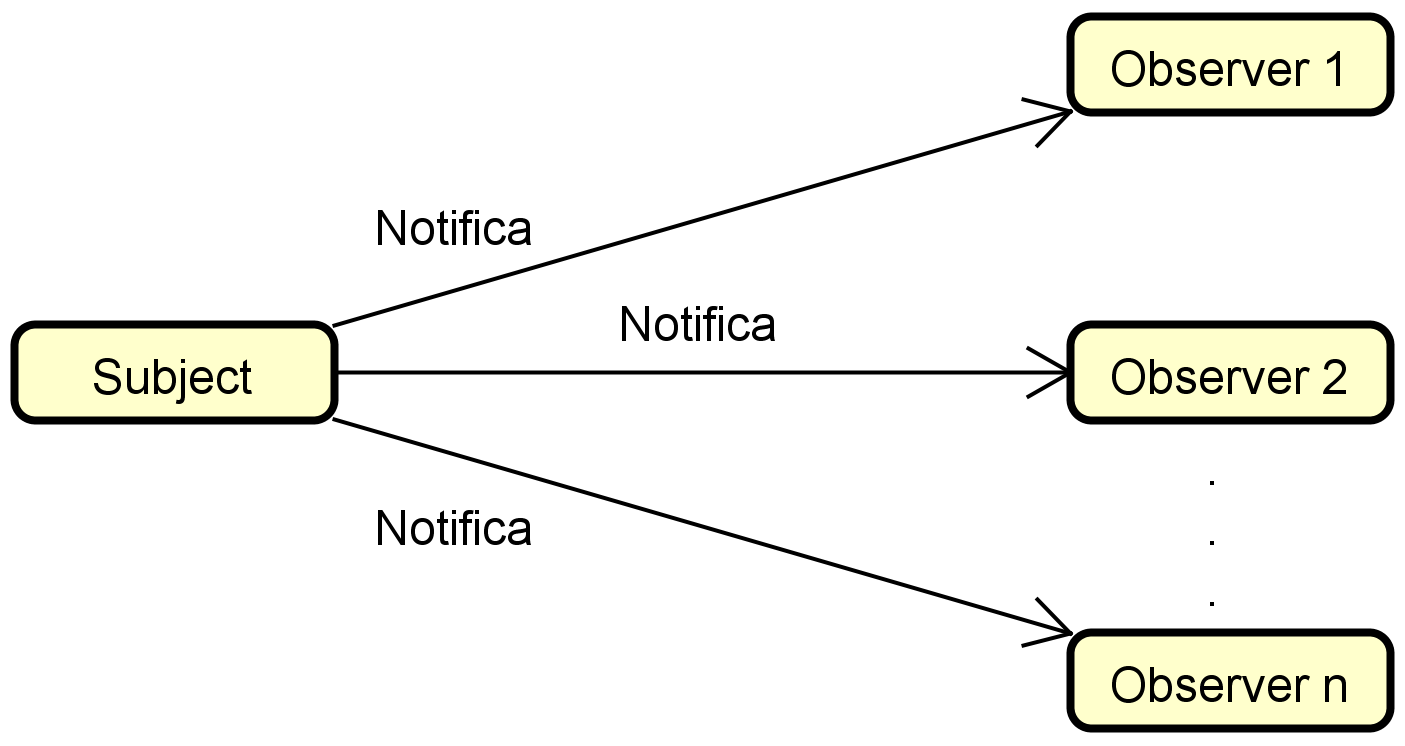
\includegraphics[scale=0.3]{Sezioni/DesignPatterns/Observer.png}
		  \caption{Schema logico del pattern Observer}
		  \end{figure}
	\item \textbf{Motivazione}: attraverso questo pattern è possibile separare le varie componenti di una applicazione web facendo sì che la parte che regola la logica dell'applicazione stessa non sappia da chi vengano emessi i vari eventi, ma sia invece in grado di recepirli e gestirli. D'altra parte, inoltre, alla parte grafica non deve interessare in seguito a che azione da parte della parte logica viene emesso un determinato evento che notifica il cambiamento di dati da mostrare, ma sia solamente in grado, utilizzando i dati trasportati con quell'evento, di aggiornarsi per mostrare tale cambiamento.
	\item \textbf{Applicabilità}: questo pattern viene utilizzato quando:
		  \begin{itemize}
		  	 	\item Si vuole poter inviare degli eventi più consistenti di quelli possibili con il pattern \termine{Event listener}.
		  	 	\item Si vuole permettere a più componenti diverse di reagire ad un determinato evento emesso da una singola componente.
		  \end{itemize}
	\item \textbf{Utilizzo}: questo pattern all'interno del progetto viene utilizzato nei seguenti casi:
		  \begin{itemize}
		  		\item Nella connessione tra l'istanza di \termine{Rocket.chat} e \progettoShort.
		  		\item Nell'interazione tra il codice HTML e la classe JavaScript associata nella sezione della \termine{View}, grazie all'utilizzo del framework \termine{Vue.js} che permette al codice \termine{Javascript} di rimanere in ascolto di eventuali interazioni da parte dell'utente con particolari oggetti HTML come i bottoni o campi di input.
		  	 	\item Nell'interazione tra \termine{View} e \termine{Presenter}, in particolare viene utilizzato per far sì che il \termine{Presenter} rimanga in ascolto (e sia pertanto l'Observer) degli eventi che si verificano all'interno della \termine{View} (che costituisce dunque il Subject) e che vengono emessi in seguito all'interazione con l'utente.
		  	 	\item Nell'interazione tra \termine{Presenter} e il database, per far sì che ogni aggiornamento che si verifica all'interno del database sia propagato correttamente anche alla parte di visualizzazione dei dati, per rendere così l'applicazione responsiva e real-time.
		  \end{itemize}
\end{itemize}

\subsection{Architetturali}
\subsubsection{Model-View-Presenter}
\begin{itemize}
	\item \textbf{Scopo}: derivato del \termine{Model-View-Controller}, questo pattern si compone di tre parti:
		  \begin{itemize}
		    	\item View: essa rappresenta la parte grafica dell'applicazione. Il suo unico scopo è inoltrare gli eventi derivati dall'interazione dell'utente con l'interfaccia grafica al Presenter, e mostrare i dati nella maniera corretta eseguendo ciò che le viene detto di fare dal Presenter. Per questo motivo essa viene definita "passiva".
		    	\item Presenter: funge da "uomo di mezzo" e serve a ricevere gli input derivanti dalla \termine{View} per eseguire di conseguenza le azioni necessarie contattando il Model. Esso inoltre rimane costantemente in ascolto del Model per eventuali cambiamenti da far visualizzare alla View.
		    	\item Model: insieme delle classi atte a modificare i dati e ad eseguire le operazioni che costituiscono la logica dell'applicazione. Esso si basa sui sistemi di persistenza dei dati come i database, e in seguito all'input derivante dai \termine{Presenter} esegue le azioni necessarie.
		  \end{itemize}	
		  \begin{figure}[H]
		  \centering
		  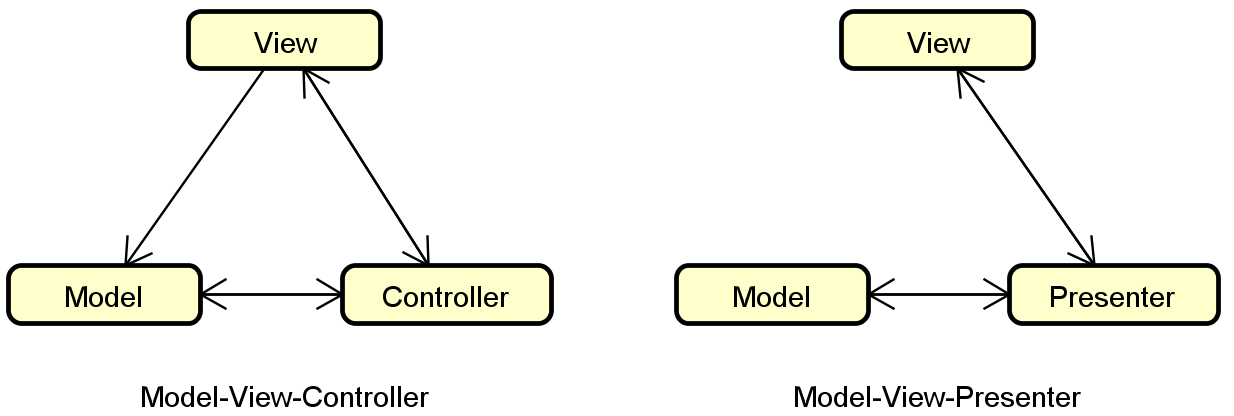
\includegraphics[scale=0.45]{Sezioni/DesignPatterns/ModelViewControllerEModelViewPresenter.png}
		  \caption{Differenza nella struttura tra pattern \termine{Model-View-Controller} e Model-View-Presenter}
		  \end{figure}	   
	\item \textbf{Motivazione}: grazie a questo pattern è possibile separare le varie componenti dell'applicazione e rendere quest'ultima più facilmente testabile. Inoltre, essendo tutte e tre le componenti indipendenti l'una dall'altra, facilita eventuali cambiamenti che potrebbero verificarsi nelle scelte architetturali durante il ciclo di vita dell'applicazione, permettendo quindi anche una maggiore manutenibilità del codice e dell'architettura stessa.
	\item \textbf{Applicabilità}: questo pattern si utilizza quando l'applicazione da realizzare possiede una componente grafica di rilevante importanza e vi è la necessità, per una migliore organizzazione, di separare le varie componenti logiche e di interfaccia grafica. Inoltre spesso viene preferita al \termine{Model-View-Controller} in quanto non vi è, come in quest'ultimo, la diretta interazione tra la parte grafica e quella logica, ma si passa invece sempre attraverso il Presenter.
	\item \textbf{Utilizzo}: all'interno di \progettoShort\ questo pattern viene utilizzato nella gestione grafica di tutte le bolle e particolari altre viste inserite all'interno dell'applicazione. Più in particolare viene adottato il seguente schema, per i widget:
\begin{itemize}
\item Le \textbf{View} saranno dei semplici template in HTML con una semplice interfaccia di comunicazione.
\item I \textbf{Presenter} verranno implementati con il design pattern comportamentale Observer, quando la View dovrà interagire con l'utente e di conseguenza il Presenter deve poter ricevere questi aggiornamenti. Se, invece, la View non deve essere aggiornata poiché statica, non verrà utilizzato il Pattern Observer, ma l'interazione sarà mantenuta solo per rimanere coerenti al Pattern e permettere una futura implementazione interattiva per chi volesse un giorno espandere l'\termine{SDK}.
\item I \textbf{Model} per i widget non saranno disponibili nell'\termine{SDK}, questo perché dovrà essere lo sviluppatore a definire il loro  comportamento, ovvero la loro \termine{Business-Logic}, mantenendo così la struttura del pattern.
\end{itemize}
Lo schema Model-View-Presenter verrà utilizzato anche nell'applicazione \app\ per ogni azione o componente.
Essendo totalmente definita e non ampliabile dallo sviluppatore (come per l'\termine{SDK}), l'applicazione definirà, oltre alla View e al Presenter, anche il Model. Quest'ultimi verranno caricati nella parte Server del programma seguendo la suddivisione logica dei programmi \textit{Meteor}.
\end{itemize}

\subsubsection{Clean Architecture}
\begin{itemize}
	\item \textbf{Scopo}: pattern simile al \termine{Model-View-Presenter} e ideato da Robert Cecil Martin, questo pattern scompone in maniera ancora più approfondita le componenti di una applicazione dividendole in quattro parti una interna all'altra, dal più esterno al più interno:
	\begin{itemize}
	  	\item Strato \textbf{esterno}: contiene i database, l'interfaccia grafica e tutte le altre componenti come framework e drivers.
	  	\item Strato \textbf{intermedio esterno}: contiene tutte quelle interfacce che permettono allo strato esterno di comunicare con quello intermedio interno. Oltre ad esse sono anche presenti le varie classi che permettono di convertire i dati dai formati utilizzati nello strato esterno a quelli utilizzati nello strato intermedio interno e viceversa.
	  	\item Strato \textbf{intermedio interno}: contiene gli \textit{use case}, ovvero quelle classi che compongono le regole logiche dell'applicazione e rappresentano il corrispettivo del Model nel modello Model \termine{View} Presenter.
	  	\item Strato \textbf{interno}: contiene tutte quelle classi che rappresentano gli oggetti che descrivono le regole logiche dell'intera azienda. Visto il loro utilizzo molto specifico, esse non verranno utilizzate nel nostro caso, di fatto rendendo questo strato per noi vuoto.
	\end{itemize}
	\begin{figure}[H]
	\centering
	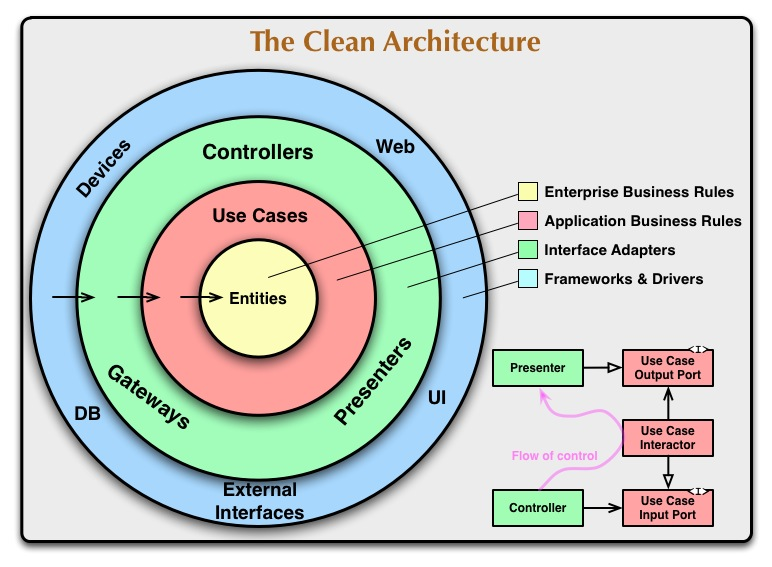
\includegraphics[scale=0.3]{Sezioni/DesignPatterns/CleanArchitecture.jpg}
	\caption{Schema a strati del pattern architetturale Clean Architecture}
	\end{figure}
	
	Oltre a questo, all'interno di questa architettura vige la \textit{dependency rule}, secondo la quale le dipendenze possono essere solamente orientate verso l'interno e di conseguenza gli strati più interni non posso dipendere da quelli più esterni. Per poter rispettare questo vincolo spesso viene utilizzato il \termine{dependency inversion principle} assieme al metodo dell'\termine{Inversion of Control} mediante \termine{dependency injection}.
	\item \textbf{Motivazione}: grazie a questo pattern è possibile dividere ulteriormente le varie componenti dell'applicazione, rendendola di conseguenza maggiormente testabile e mantenibile. Oltre a ciò, grazie ai vari adapter posti tra uno strato e l'altro, essa permette di rendere i vari strati esterni indifferenti ad eventuali cambiamenti negli strati più interni e viceversa.
	\item \textbf{Applicabilità}: questo design pattern viene utilizzato quando si vuole creare una applicazione che sia, in ogni suo componente, facilmente modificabile senza dover andare a riscrivere grandi quantità di codice. Esso viene particolarmente in aiuto nello sviluppo di applicazioni che utilizzano vari framework, librerie e componenti di terze parti propense a cambiare nel tempo e che devono poter rispondere a tali cambiamenti in maniera rapida ed efficace.
	\item \textbf{Utilizzo}: questo design pattern viene utilizzato nello sviluppo dell'applicazione demo, in particolare nella gestione delle bolle e della logica ad esse connesse, oltre che alla creazione dell'interfaccia grafica e della logica di eventuali altre viste in essa presenti. E' stato scelto questo tipo di architettura poiché funziona molto bene con il pattern MVP e poiché suddivide bene gli strati, i loro ingressi e le loro uscite. Inoltre come riferito nel \textit{Verbale interno} del 26 Febbraio 2017 ed in particolare nella decisione \textit{VI4.3}, gli strati sono i seguenti:
\begin{itemize}
\item Il primo è lo strato più esterno e gestisce la comunicazione con tutto ciò che non è interno all'applicazione.
\item Il secondo fa riferimento ai vari presenter che fanno da tramite tra il Model e la View.
\item Il terzo fa riferimento alla \termine{Business Logic}, ovvero ai model.
\item Il quarto rappresenta il database.
\end{itemize}
\end{itemize}
 
\end{appendices}
\end{document}